\section{Results}
\label{sec:resu}

An evenly sampled output of a jitter-less \emph{RO} was simulated with Matlab\textsuperscript{\copyright} and an output file with a length of $N_b=7,000,000$ of bits was generated. A set of a hundred values of the sampling ratio $r= T_s/T\in[6.5,9.5]$, was explored (where $T_s$ is the sampling period and $T$ is the \emph{RO}  output period). Jitter with a normal distribution and a set with different values of variance $\sigma_s$ (see below) were added to the original file. Our method emulates the real process of sampling the noisy output of a real \emph{RO}; the detailed code is published in Mathworks\cite{MathworksMaxi}.

For each value of $\sigma_s$, ten surrogates (each one with a different random initial condition) were generated and new files with $N_b$ bits each were stored. It was assumed that jitter of individual samples is independent, normal distributed random variables, with zero mean value and variance $\sigma_i=\sigma_s$. Consequently, the variance of the accumulated jitter over one period $T$ is given by $\sigma^2_T=r \sigma^2_s$ \cite{Valtchanov2008}. The values considered  are $\sigma_T=\{0,$ $0.001,$ $0.002,$ $0.003,$ $0.004,$ $0.005,$ $0.007,$ $0.01,$ $0.02,$ $0.02,$ $0.04,$ $0.05,$ $0.07,$ $0.1\}$.

For each file all the quantifiers defined in \ref{sec:quanti} were evaluated for $D\in[2,10]$ and $W\in[1,26]$. The details about evaluation, advantages and drawbacks of each quantifier are reported in section \ref{sec:quanti}: they are $S_W$, $S^{(D)}_{BP}$, $H_{W}$, $H^{(D)}_{BP}$, $h$ and $h^*$.  Let us only show here the  more relevant results  to show the reason the last two quantifiers ($h$ and $h^*$) are the best ones.

\begin{itemize}
\item In the case of normalized entropy $H_{W}$, it strongly depends on $W$. Furthermore the analysis of $H_{W}$ as a function of $r$ shows that it does not allow to determine an optimum value of the sampling ratio $r$ (see Fig. \ref{fig:H_W_rCS}). This is an important issue if the quantifiers are going to be used for experimental setups. 
\item In the case of the normalized Bandt \& Pompe entropy $H^{(D)}_{BP}$, a strong dependence on the embedding dimension $D$ is additionally present. Again it is not easy to determine the optimum value of $r$ from the analysis of this parameter as a function of $r$  (see Fig. \ref{fig:HBP_W_rSS}). 
\item A similar behavior appears in all the other functionals related with these two entropies. 
In summary, our results show that  both $ h$ y $h^*$ are independent of any arbitrary parameter used in their statistical determination.  These two quantifiers have also been considered in two excellent articles \cite{Amigo2006,Ebeling2001}. 
\end{itemize}
%
\begin{figure}
\center
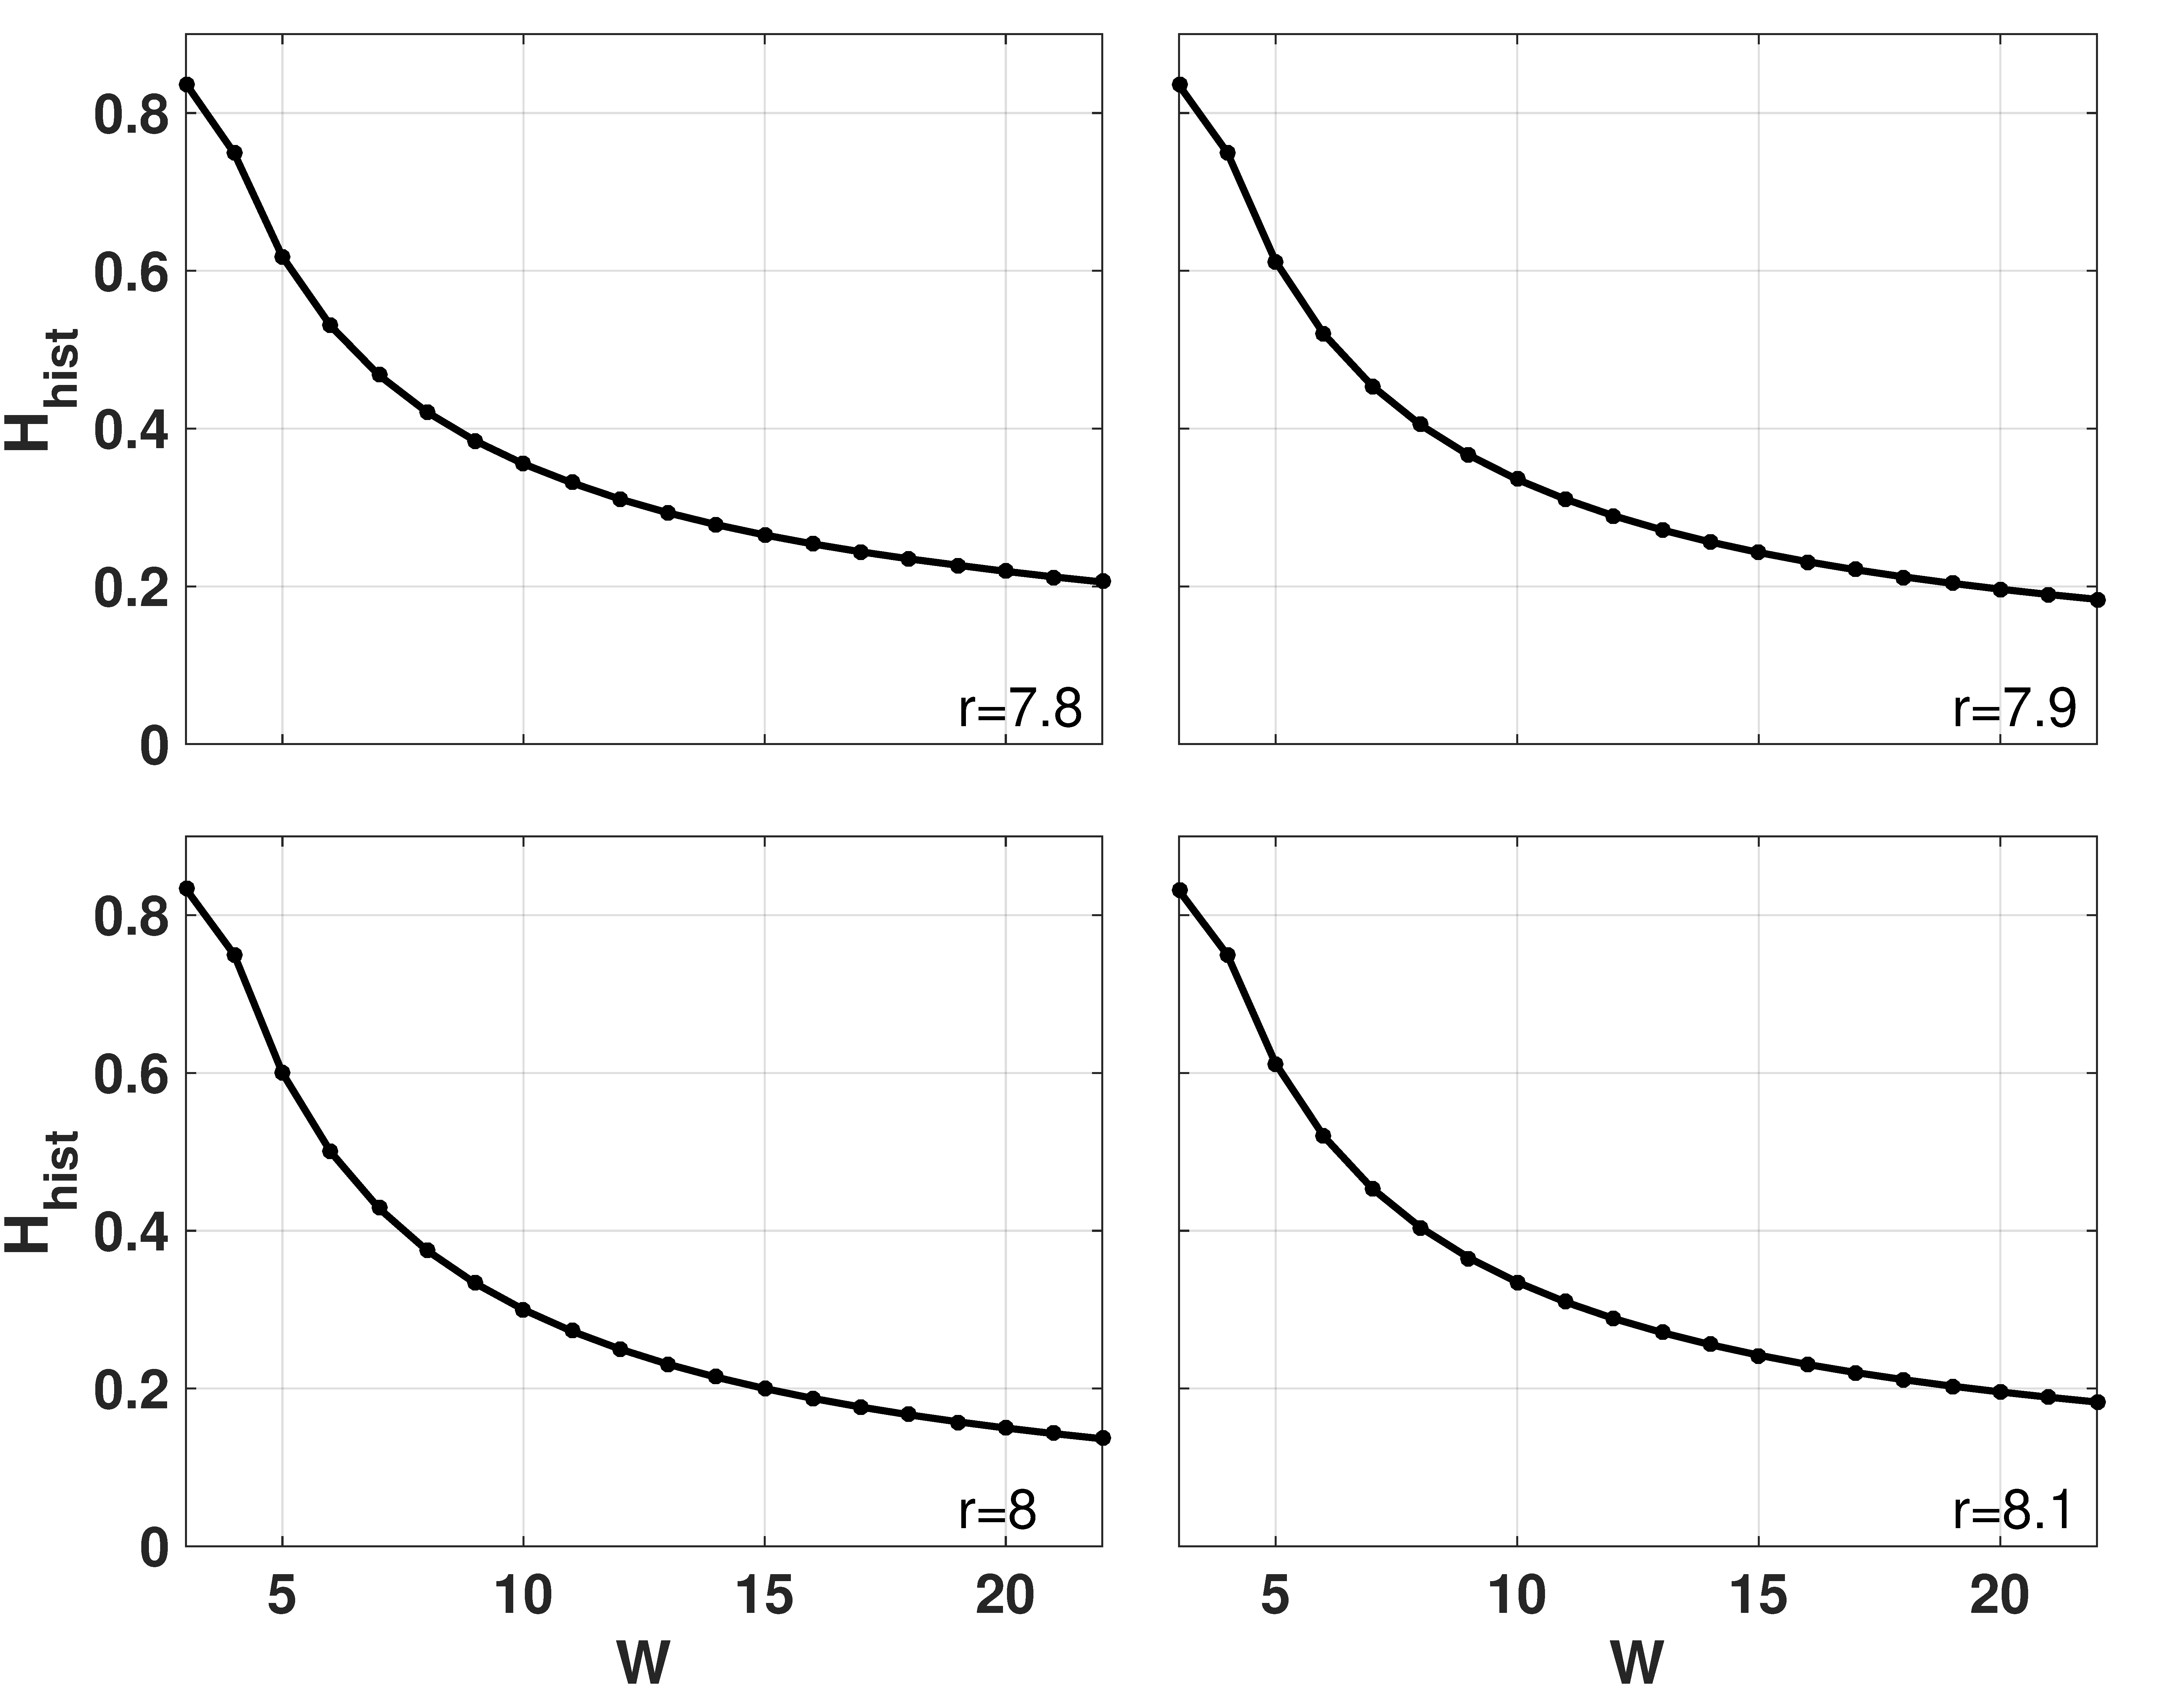
\includegraphics[width=0.8\textwidth]{H_W_rCS}
\caption{Normalized entropy $H_W$ as a function of $W$ for a jitter-less \emph{RO} sampled with different values of $r$.}
\label{fig:H_W_rCS}
\end{figure}
%
\begin{figure}
\center
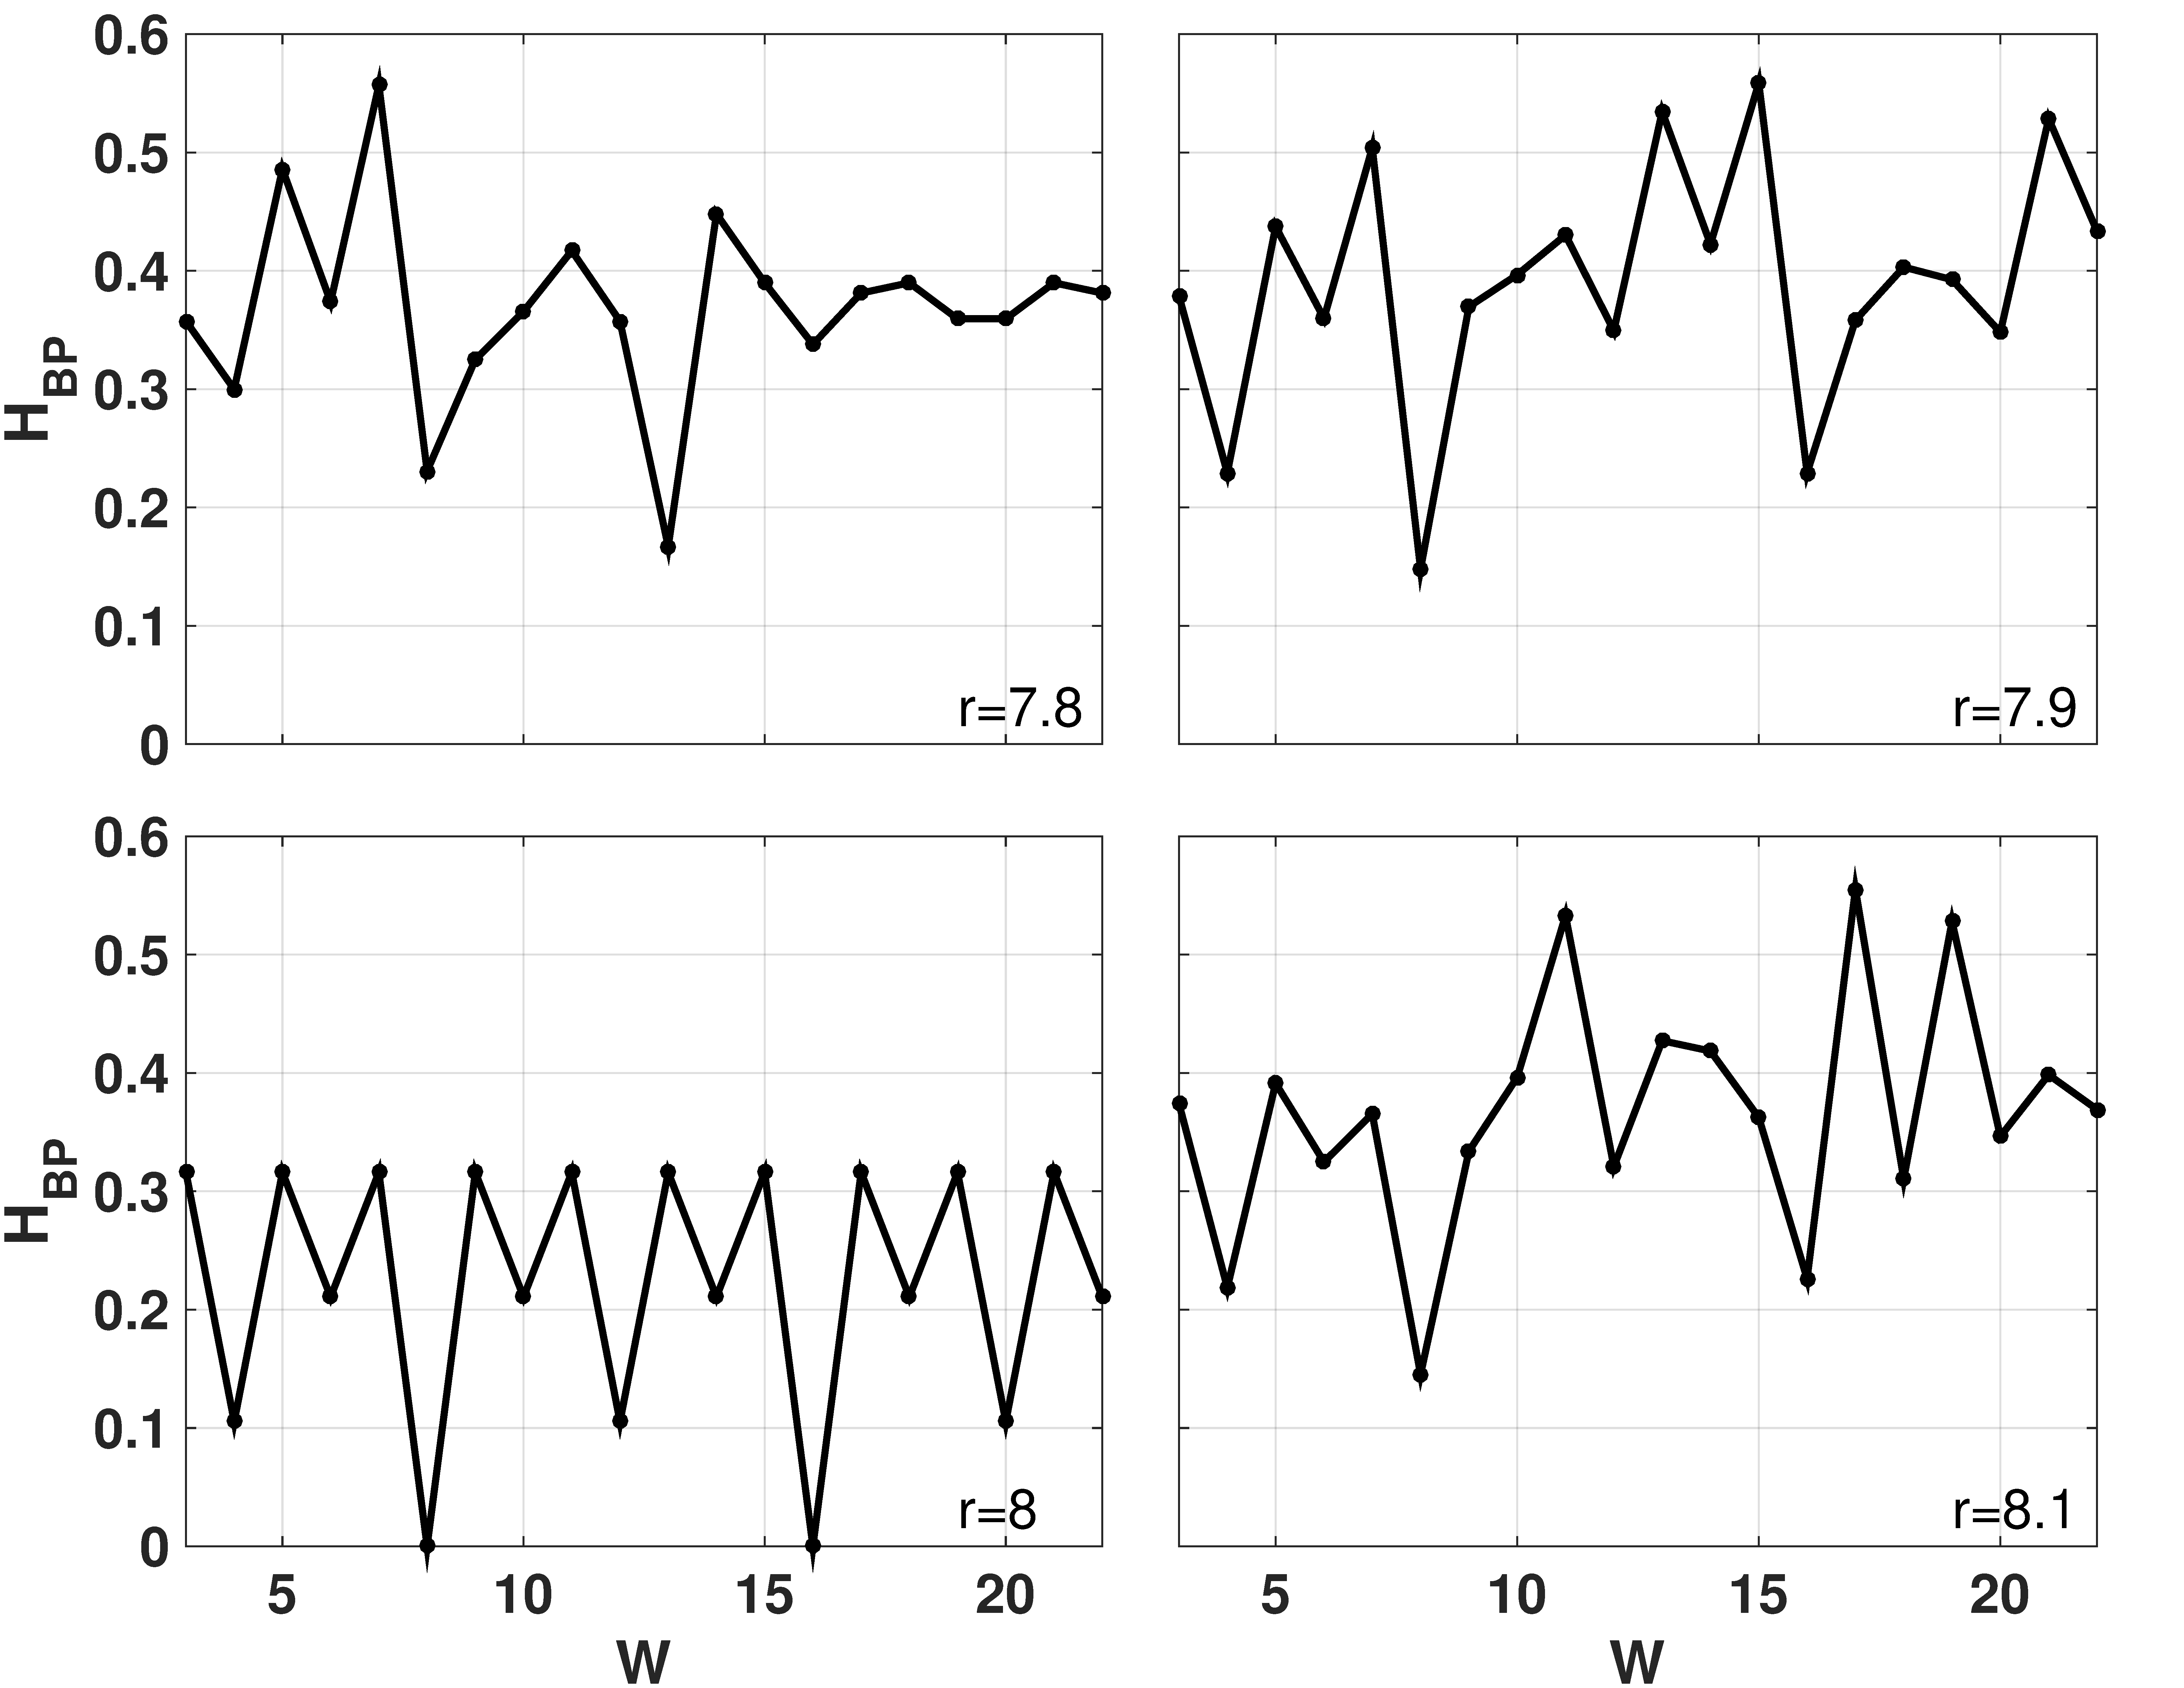
\includegraphics[ width=0.8\textwidth]{HBP_W_rSS}
\caption{$H^{(D)}_{BP}$ as a function of $W$ for a jitter-less \emph{RO} sampled with different values of $r$. Calculations are made without superposition of words}
\label{fig:HBP_W_rSS}
\end{figure}

Our results show that two quantifiers, $h$ and $h^*$, are appropriate to be used as jitter measures because: 
\begin{itemize} 
\item (a) for $\sigma_T=0$ (jitter-less output) they rapidly approach to a constant limiting value as both $D$ and $W$ increase toward $\infty$ and this limiting value is independent of both $D$ and $W$; 
\item (b) they are increasing monotone (and almost proportional) functions of $\sigma_T$. \item (c) From their analysis, it is possible to detect the optimum value of the sampling ratio $r$. Let us show these claims in the following figures that are representative of all our results. 
\end{itemize}
%
Figure \ref{fig:hm_D_SJ} shows the Bandt \& Pompe differential entropy $h^*$, as a function of $D$, with $W$ as a parameter, for a ring without jitter. It can be seen that there is a threshold value $W=4$ over which all the curves collapse into one for every value of $D$. Furthermore, Fig. \ref{fig:hm_D_SJ} also shows that for $D\ge8$ all the curves collapse into one, regardless the value of $W$. In conclusion, if $D\ge 8$ and $W\ge 4$ one obtains a quantifier independent of both $D$ and $W$. The influence of jitter on this quantifier is shown in Figure \ref{fig:hm_D_CJ}, where $h^*$ is plotted as a function of $D$ with $\sigma_T$ as a parameter. The values considered are $\sigma_T=\{0 (no~jitter),$ $0.001,$ $0.002,$ $0.003,$ $0.004,$ $0.005,$ $0.007,$ $0.01,$ $0.02,$ $0.02,$ $0.04,$ $0.05,$ $0.07,$ $0.1\}$. The inset of Fig. \ref{fig:hm_D_CJ} shows $h^*$ as a function of $\sigma_T$ for $D=8$. This inset shows that this quantifier is an increasing monotone function of $\sigma_T$. Finally Fig. \ref{fig:hm_r_CJ} shows $h^*$ as a function of the sampling ratio $r$. 
In this figure, it is shown that there is a minimum for the right $r$ (in this case $r=8$). Furthermore sensitivity of $h^*$ as a function of jitter is maximum for this same ideal value of $r$.

\begin{figure}
\center
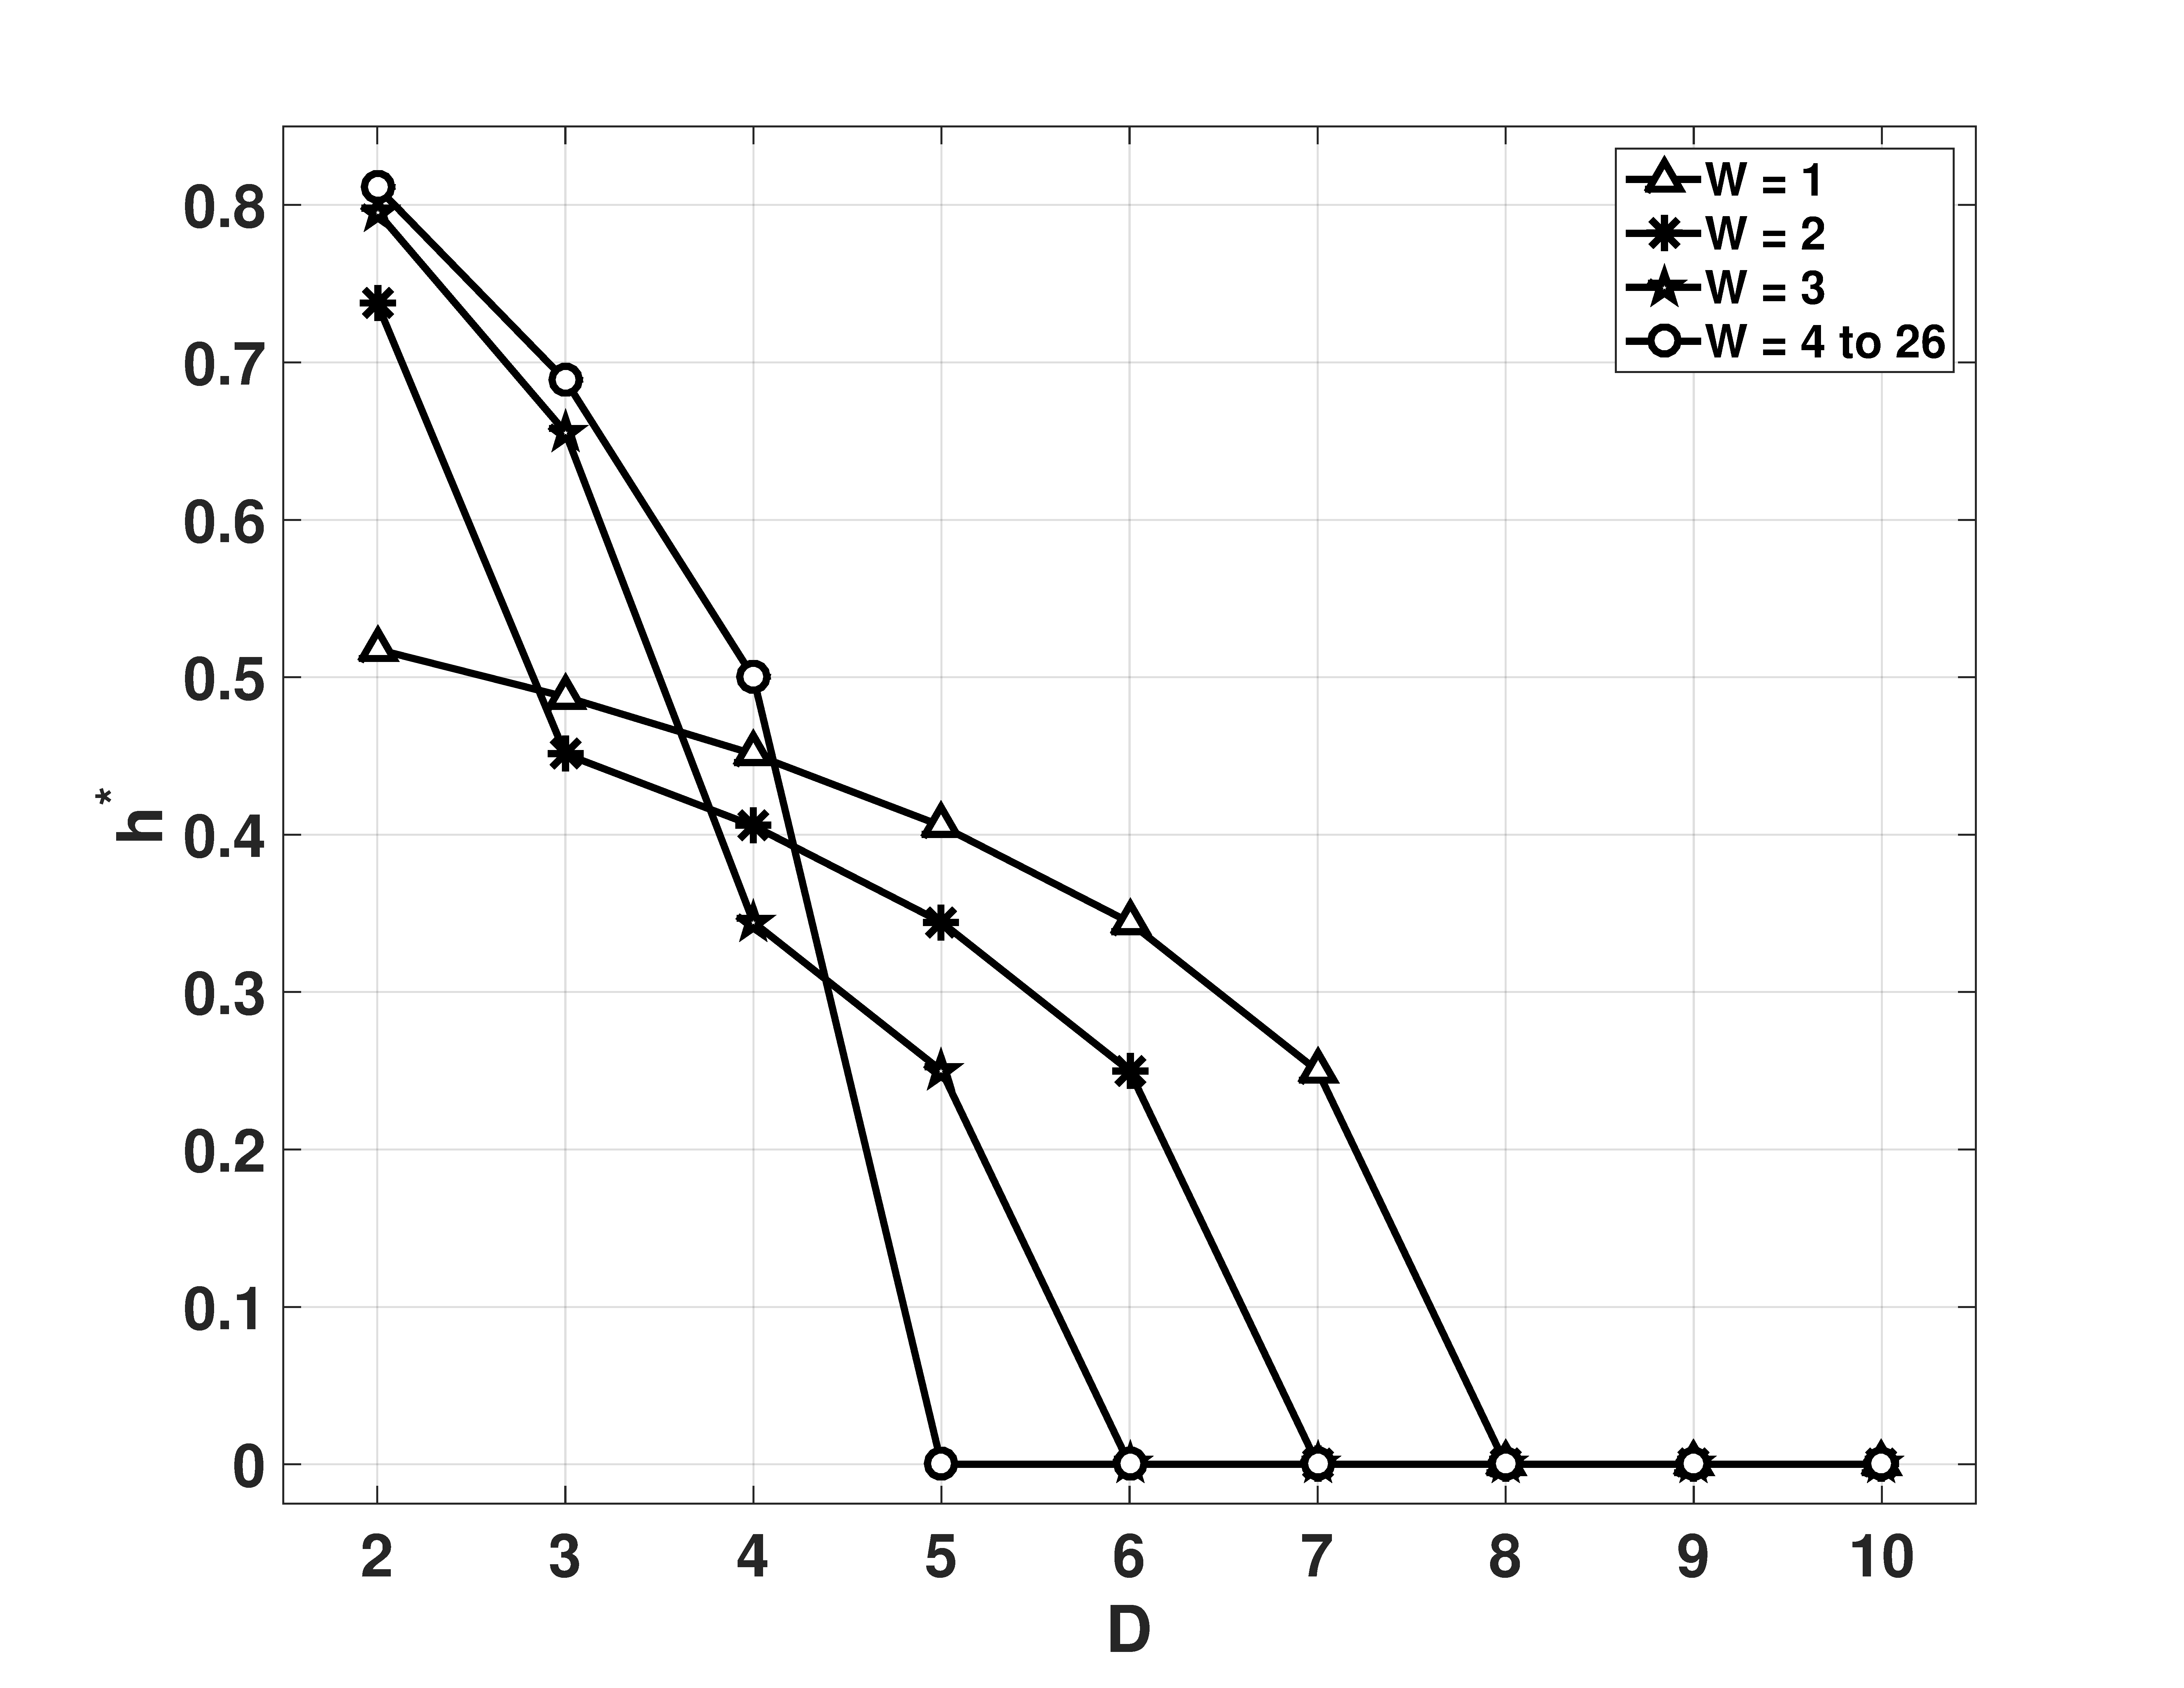
\includegraphics[ width=0.8\textwidth]{hm_D_SJ}
\caption{$h^*$ as a function of $D$ for a jitter-less \emph{RO} sampled with $r=8$.}
\label{fig:hm_D_SJ}
\end{figure}

\begin{figure}
\center
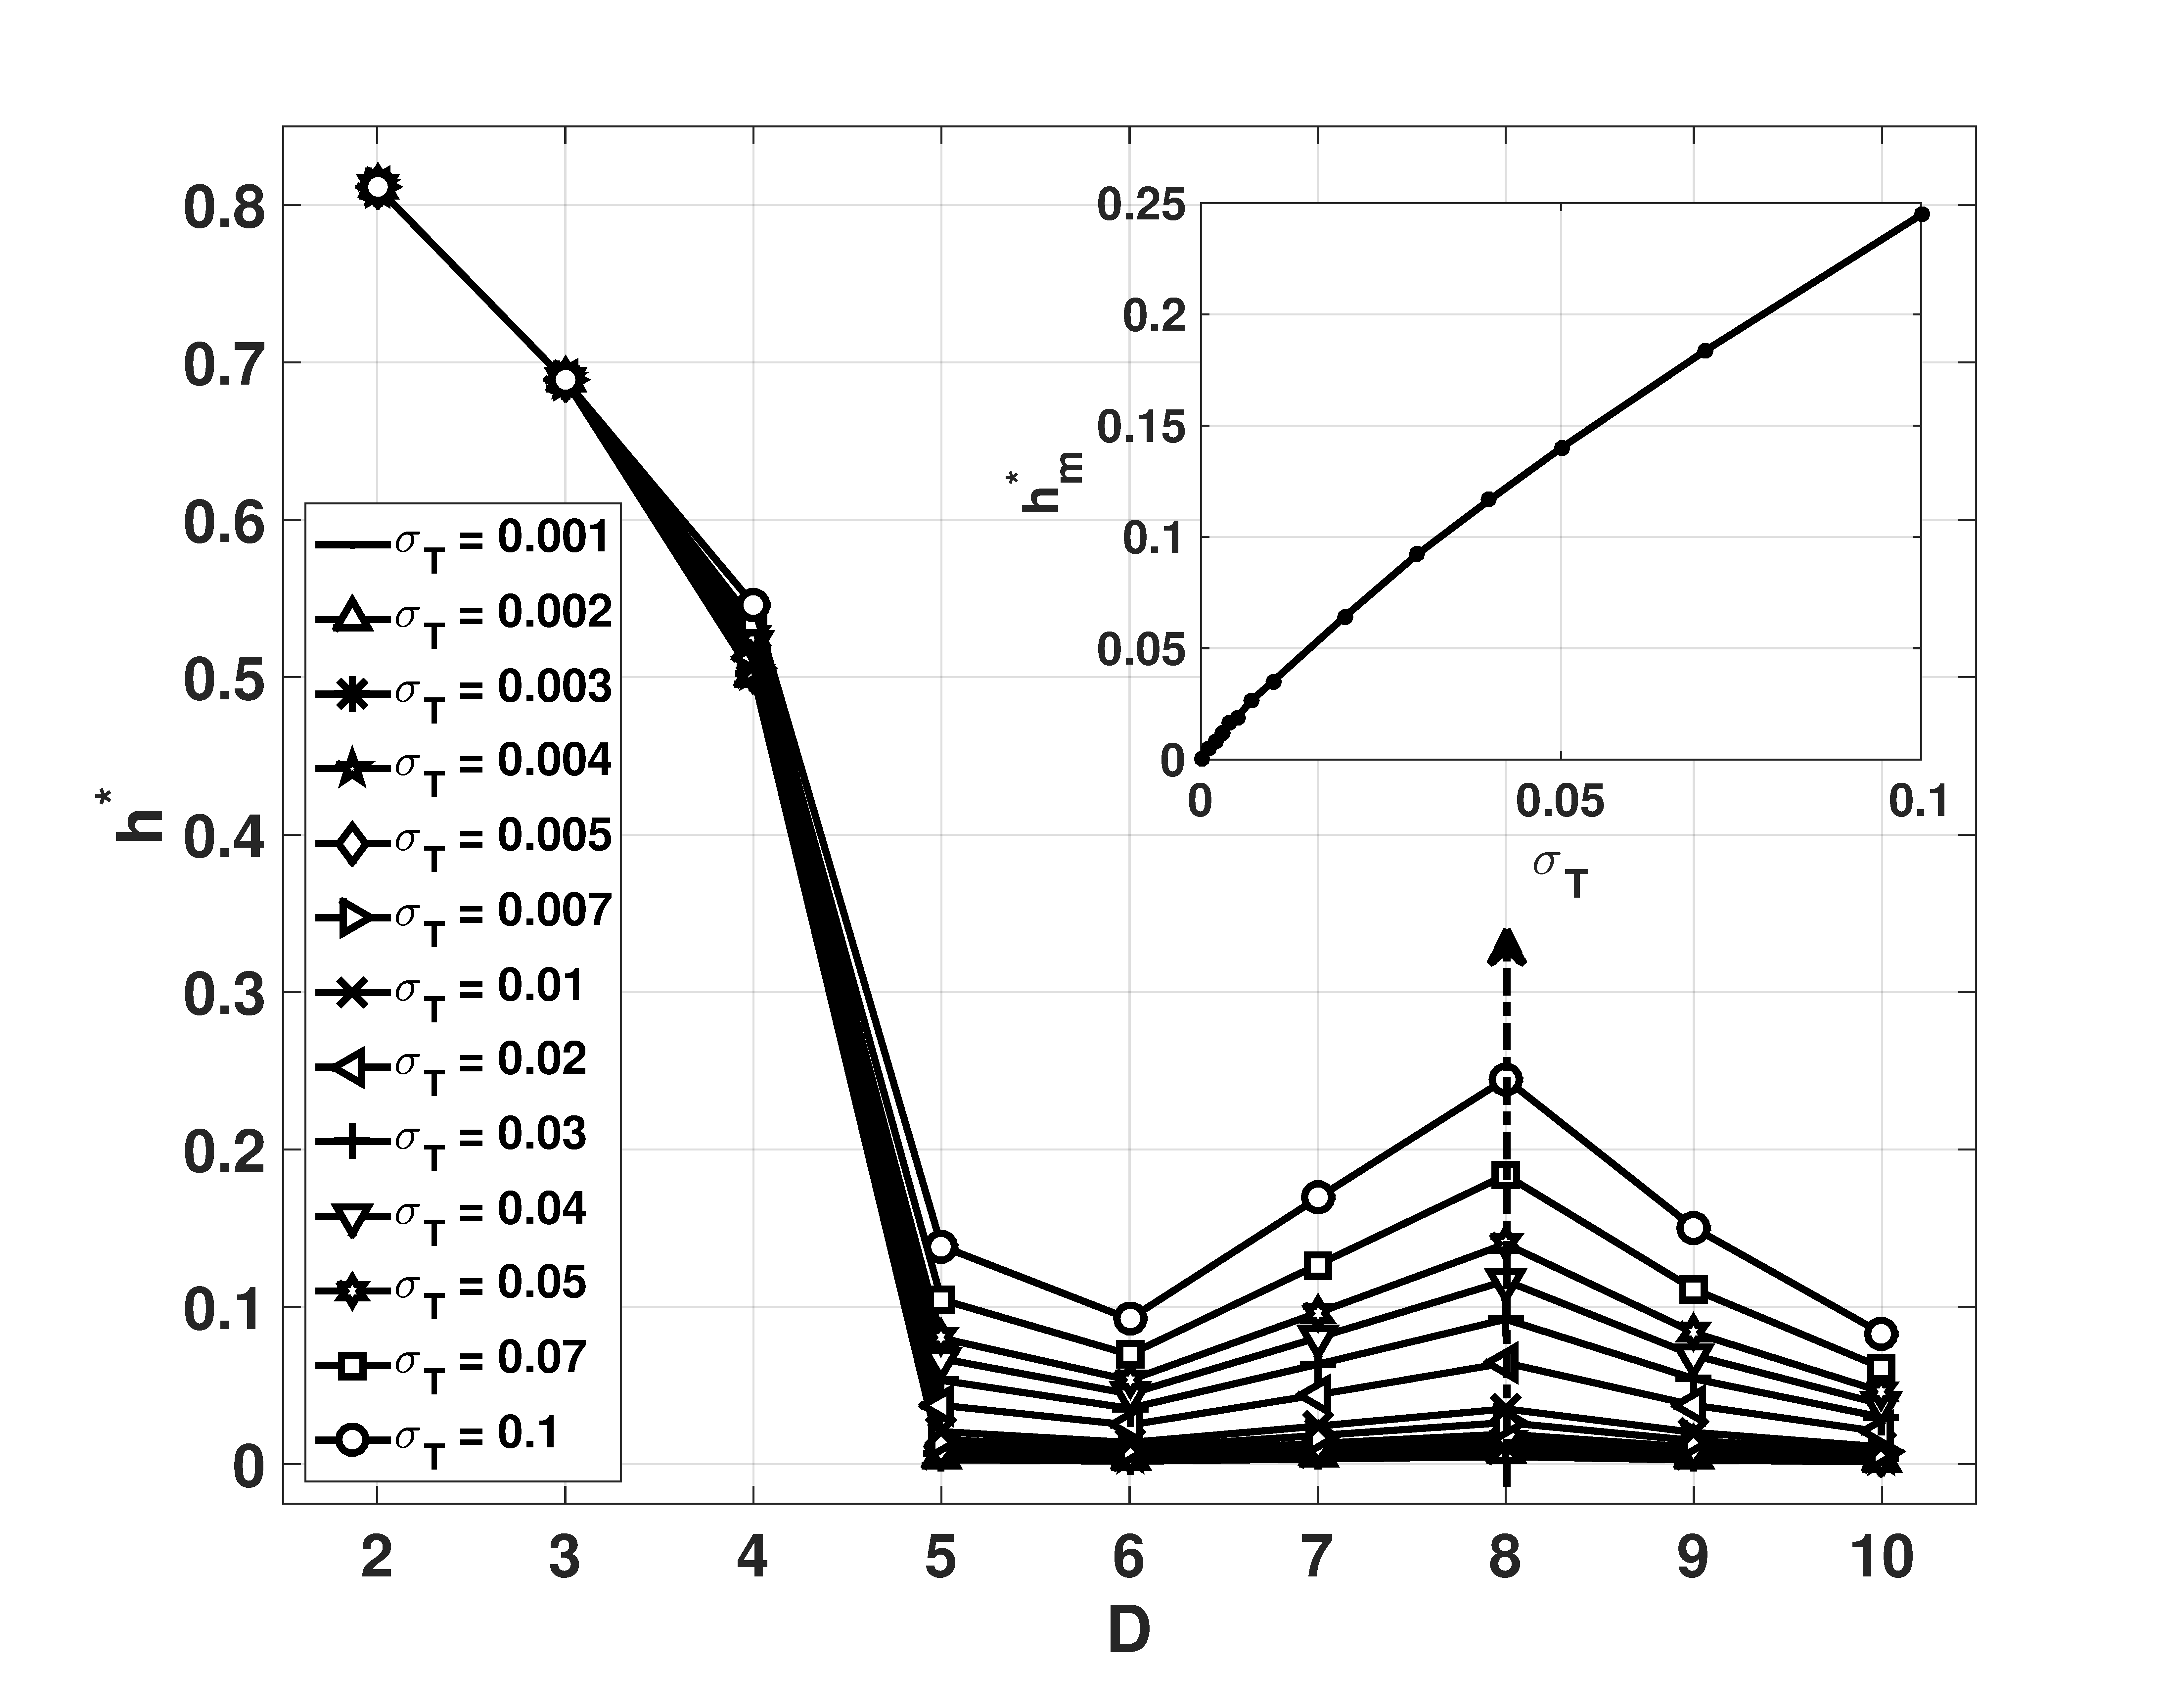
\includegraphics[width=0.8\textwidth]{hm_D_CJ}
\caption{$h^*$ as a function of $D$ for a \emph{RO} sampled with $r=8$ for a world length $W=6$ for jitter with several variances. The inset shows $h^*$ as a function of $\sigma_T$ for $r=8$, $W=6$ and $D=8$.}
\label{fig:hm_D_CJ}
\end{figure}

\begin{figure}
\center
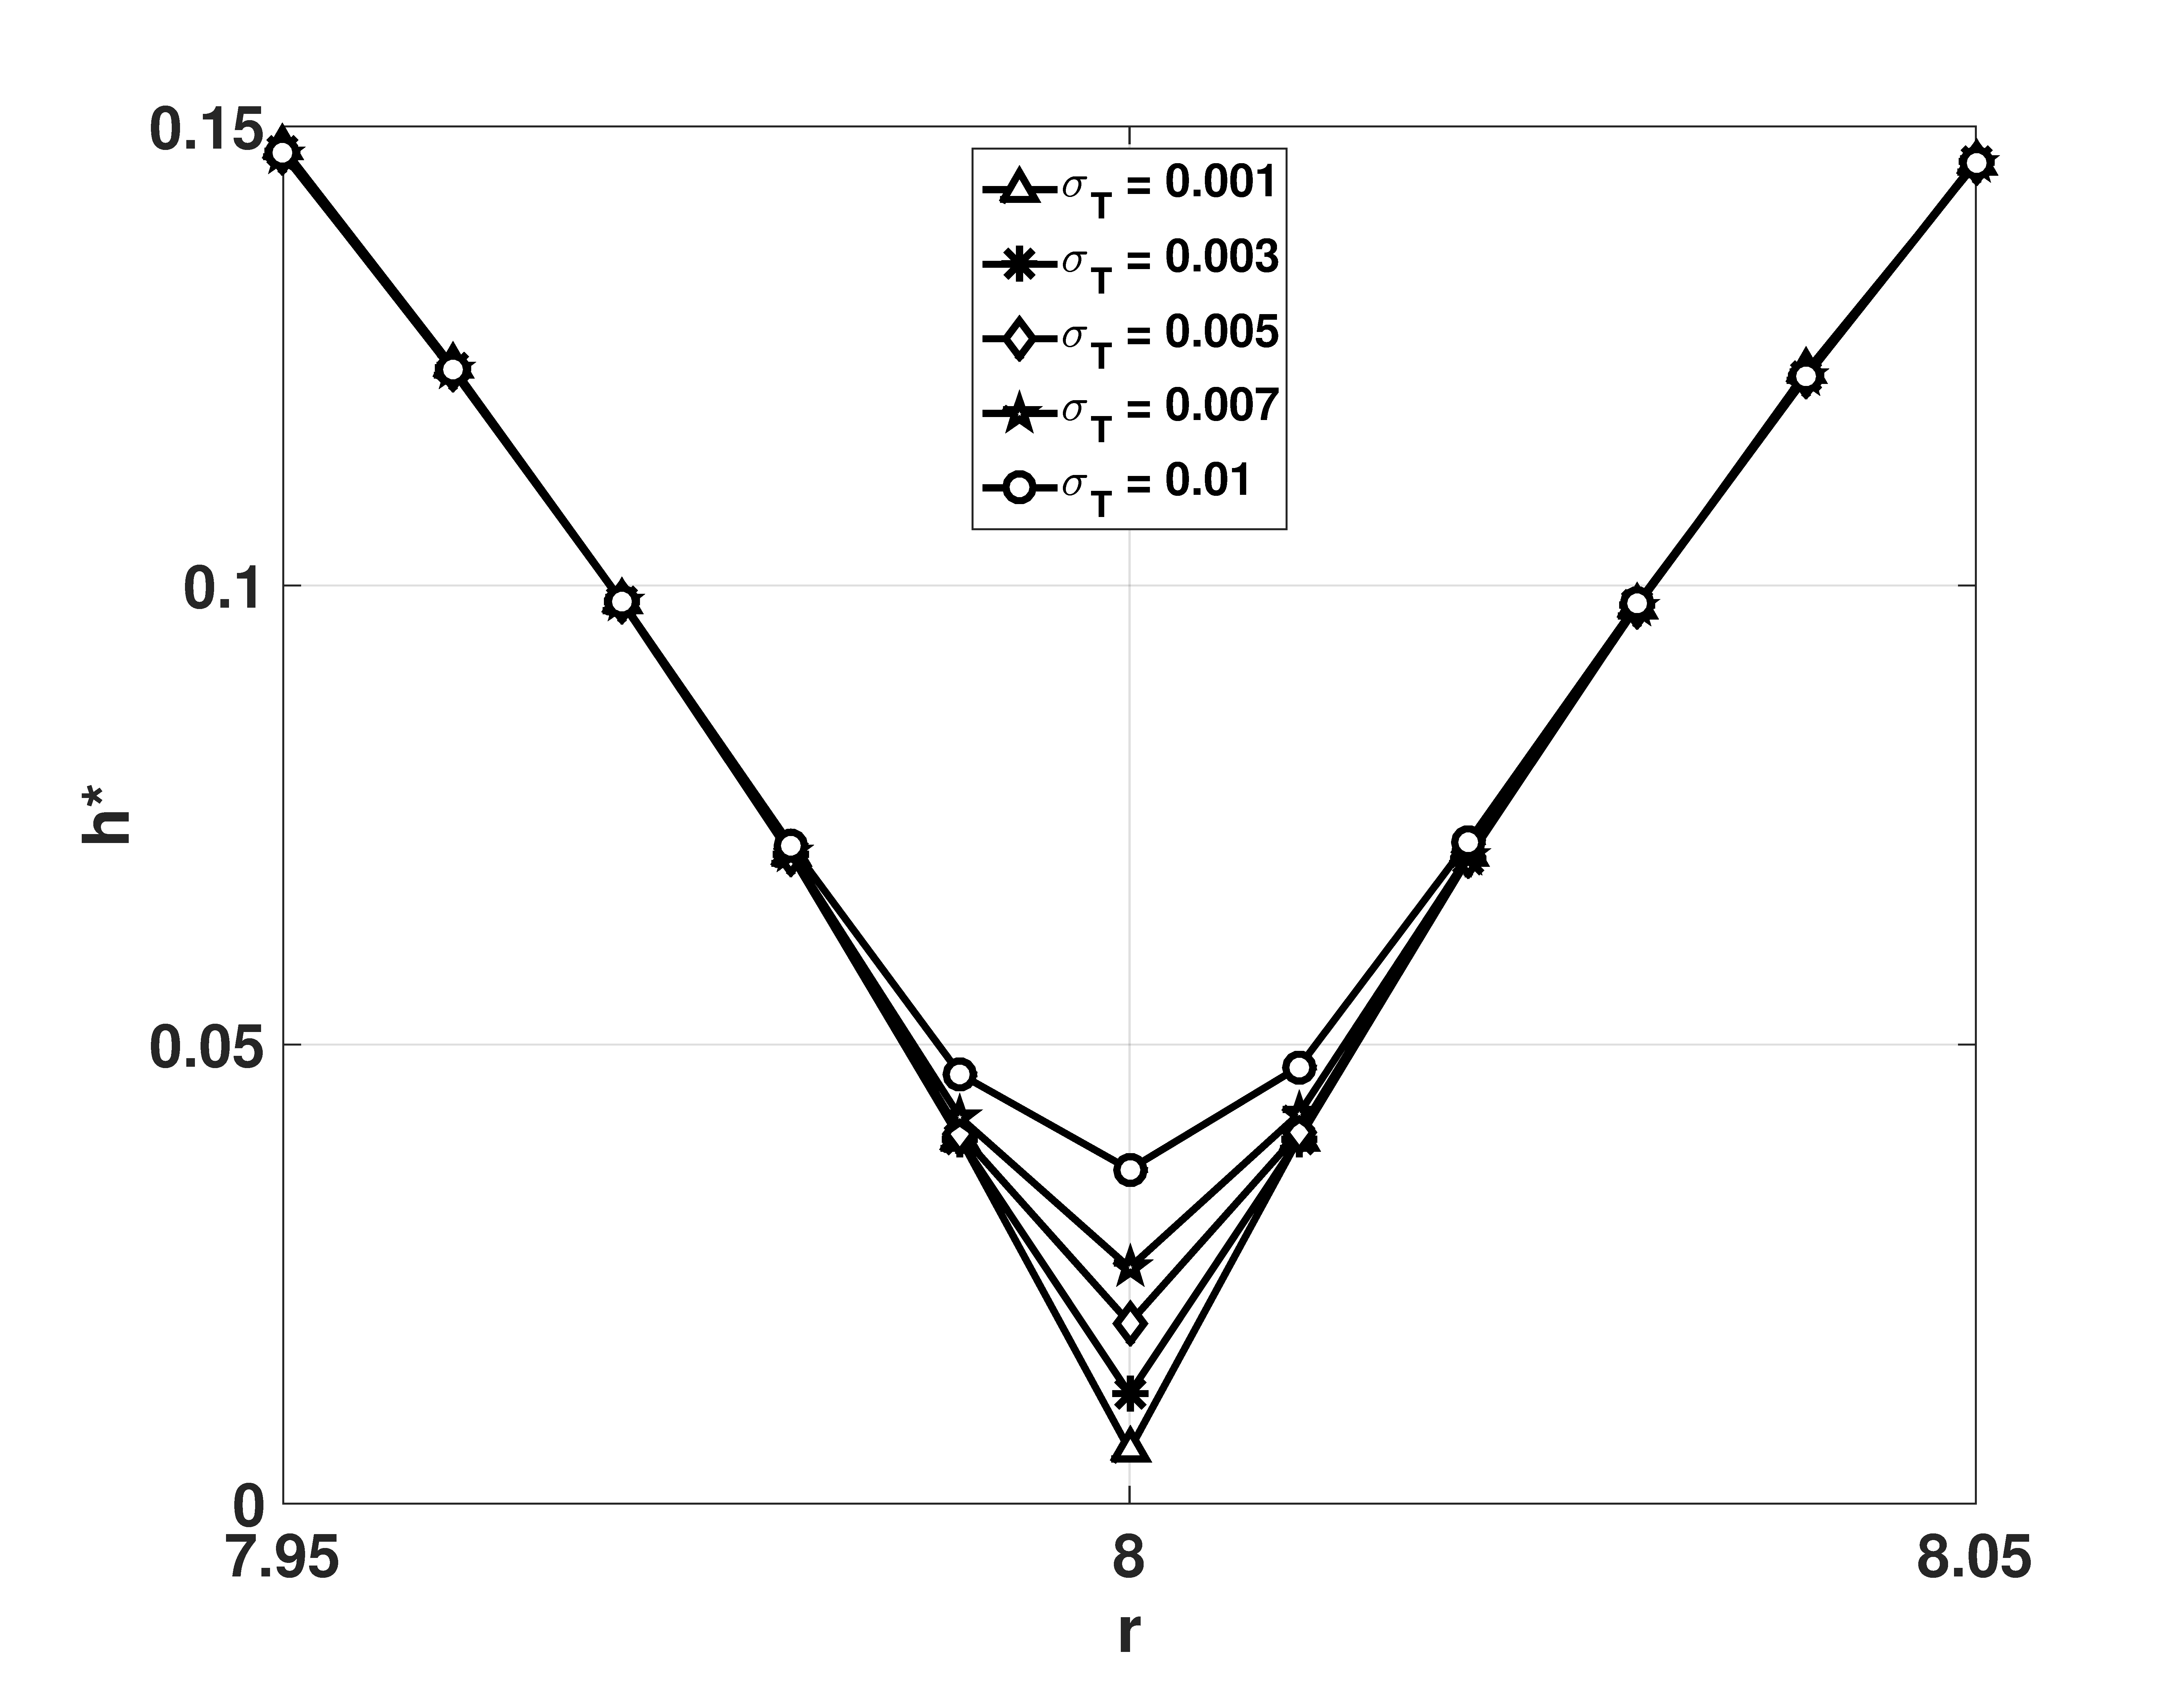
\includegraphics[ width=0.8\textwidth]{hm_r_CJ}
\caption{$h^*$ as a function of $r$ for $r\in[7.95,8.05]$, with several $\sigma_T$, $W=6$ and $D=8$. The curve has a minimum at the correct value $r=8$.}
\label{fig:hm_r_CJ}
\end{figure}

Let us now analyze the second quantifier, $h$. This quantifier only depends on $W$ because $D$ is not used to define the \emph{PDF} assigned to the data series. Fig. \ref{fig:h_W_SJ} shows jitter-less case, $h$ is almost independent of $W$ for $W\ge4$. In this paper, we adopted $W=6$. Figure \ref{fig:h_W_CJ} shows the influence of jitter over this quantifier. It is clear from the inset in this figure that, for the selected value $W=6$, $h$ is an increasing monotone function of jitter variance $\sigma_T$.

Fig. \ref{fig:h_r_CJ} shows that $h$ has a minimum when the value of $r$ takes its optimum value ($r=8$). Note that this minimum is robust also in the presence of jitter.

\begin{figure}
\center
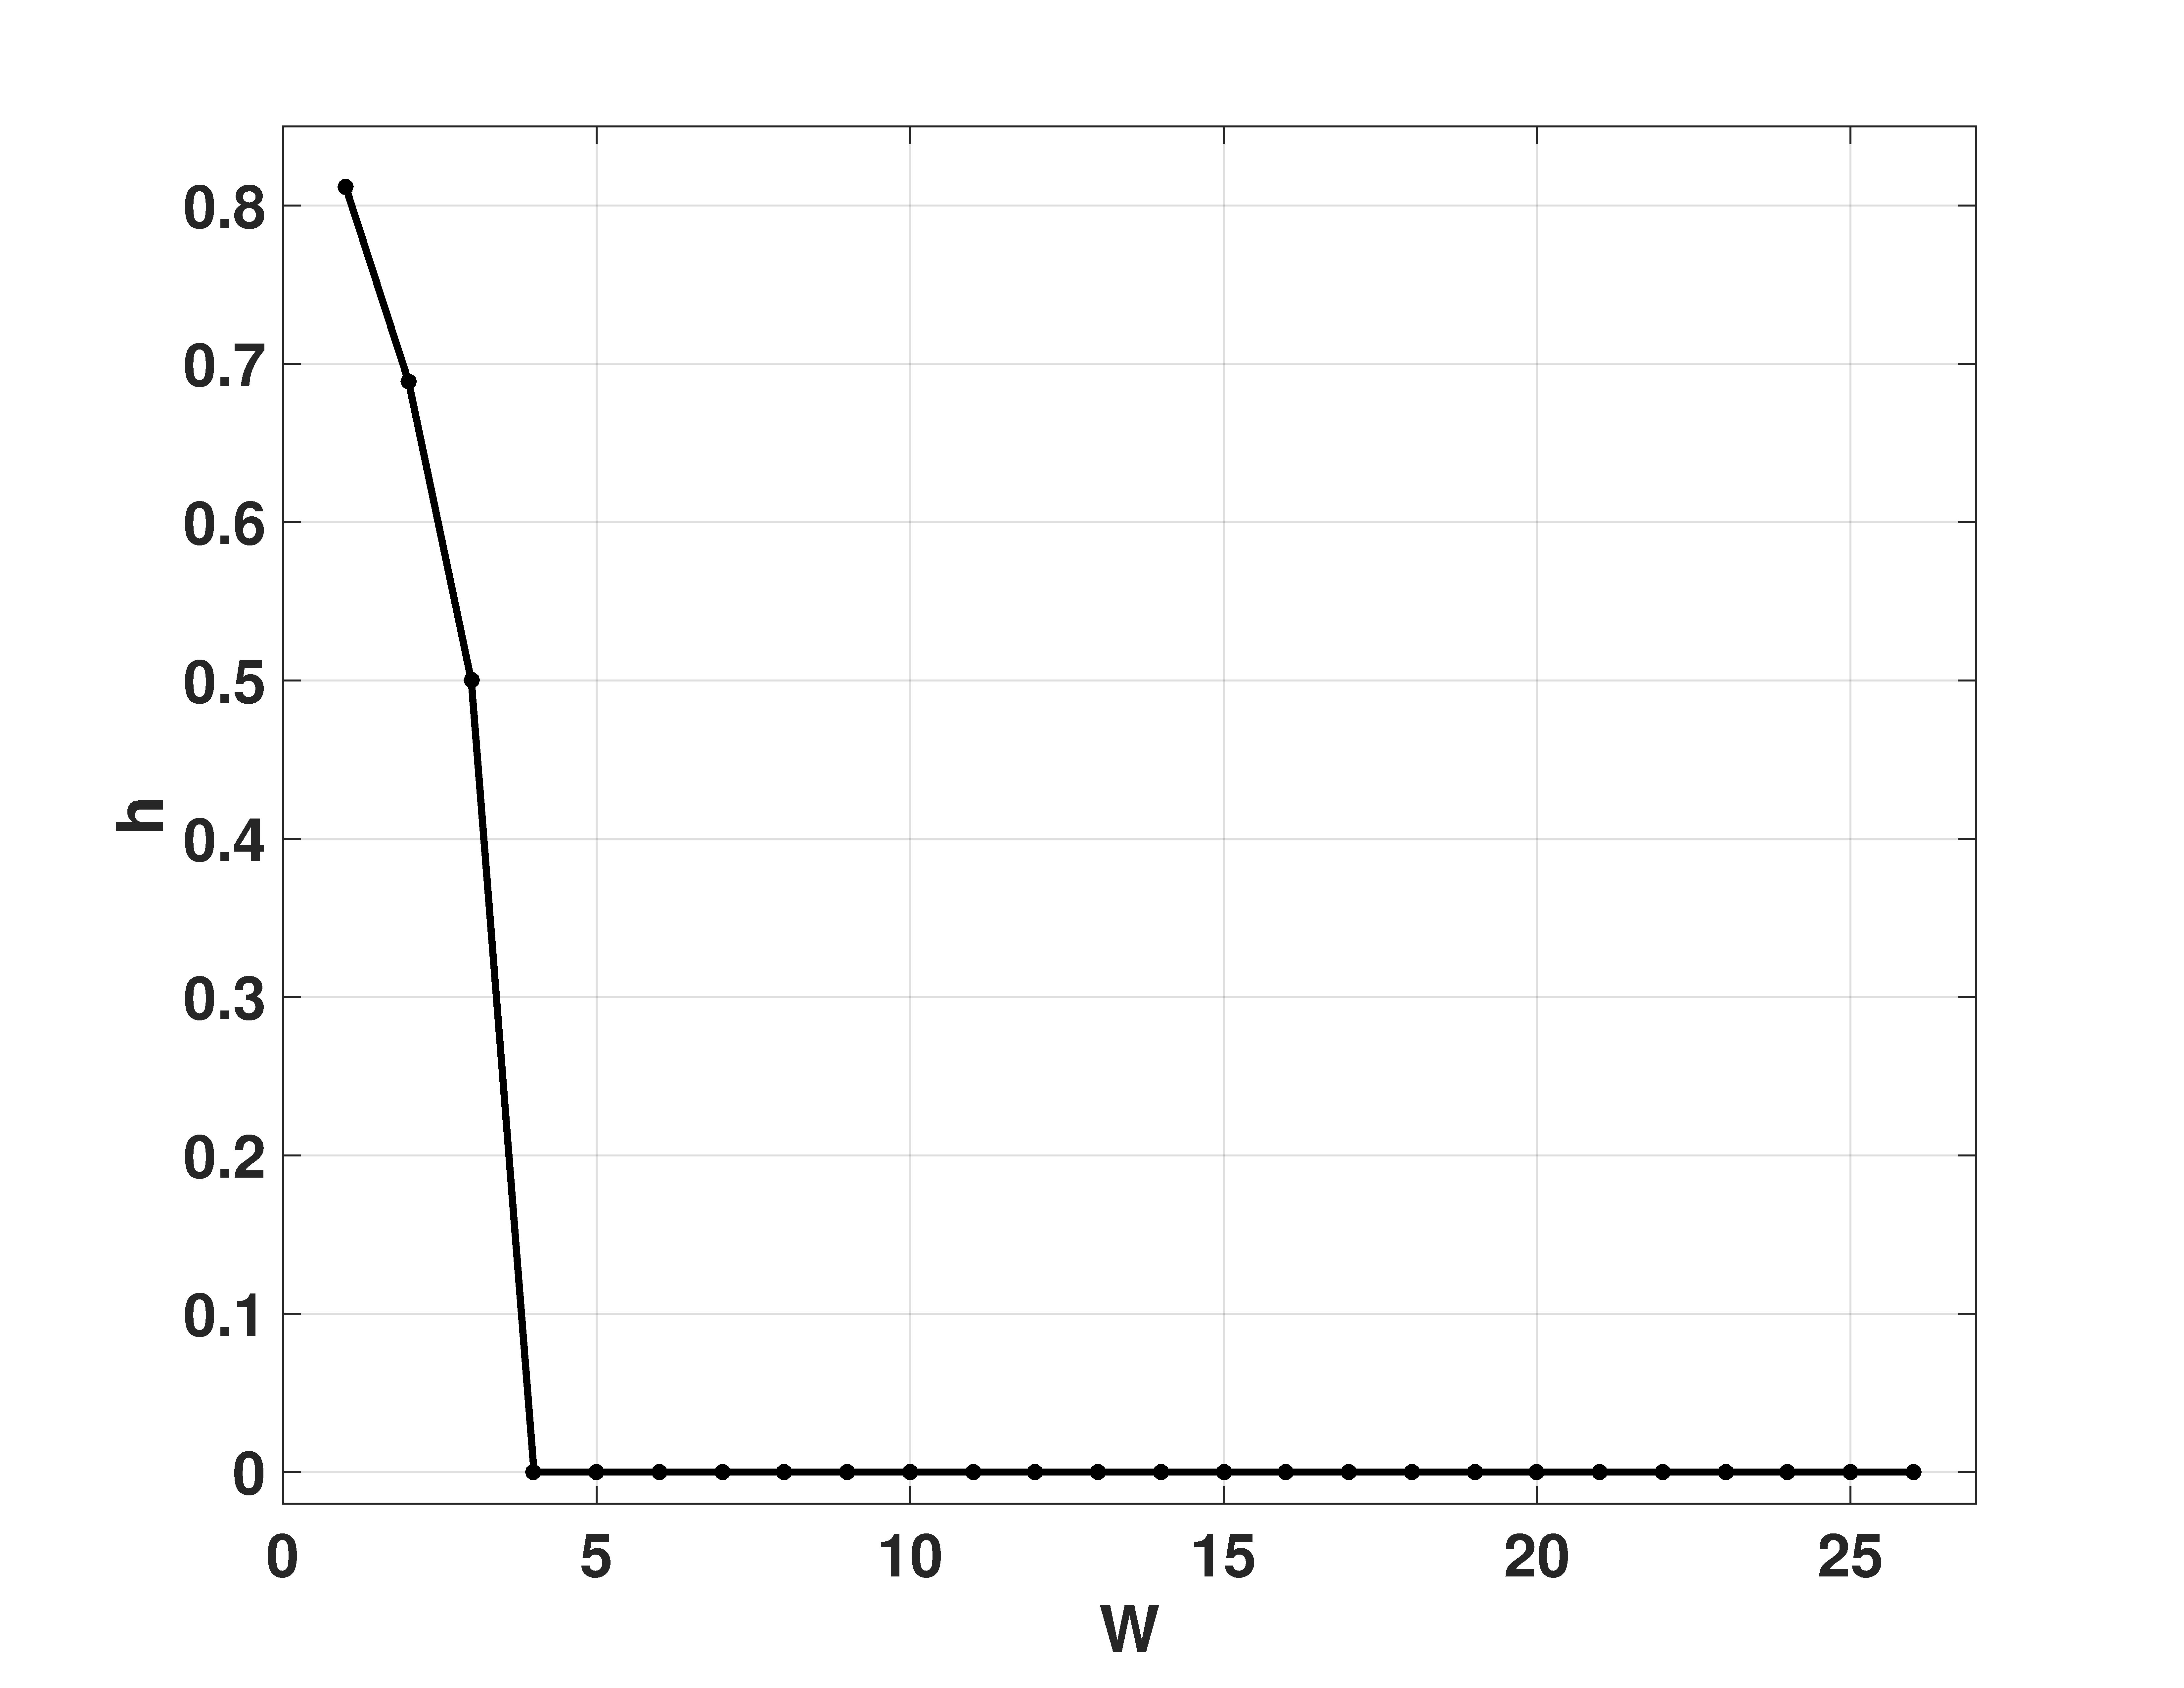
\includegraphics[width=0.8\textwidth]{h_W_SJ}
\caption{$h$ as a function of $W$ for a jitter-less \emph{RO} sampled with $r=8$.}
\label{fig:h_W_SJ}
\end{figure}

\begin{figure}
\center
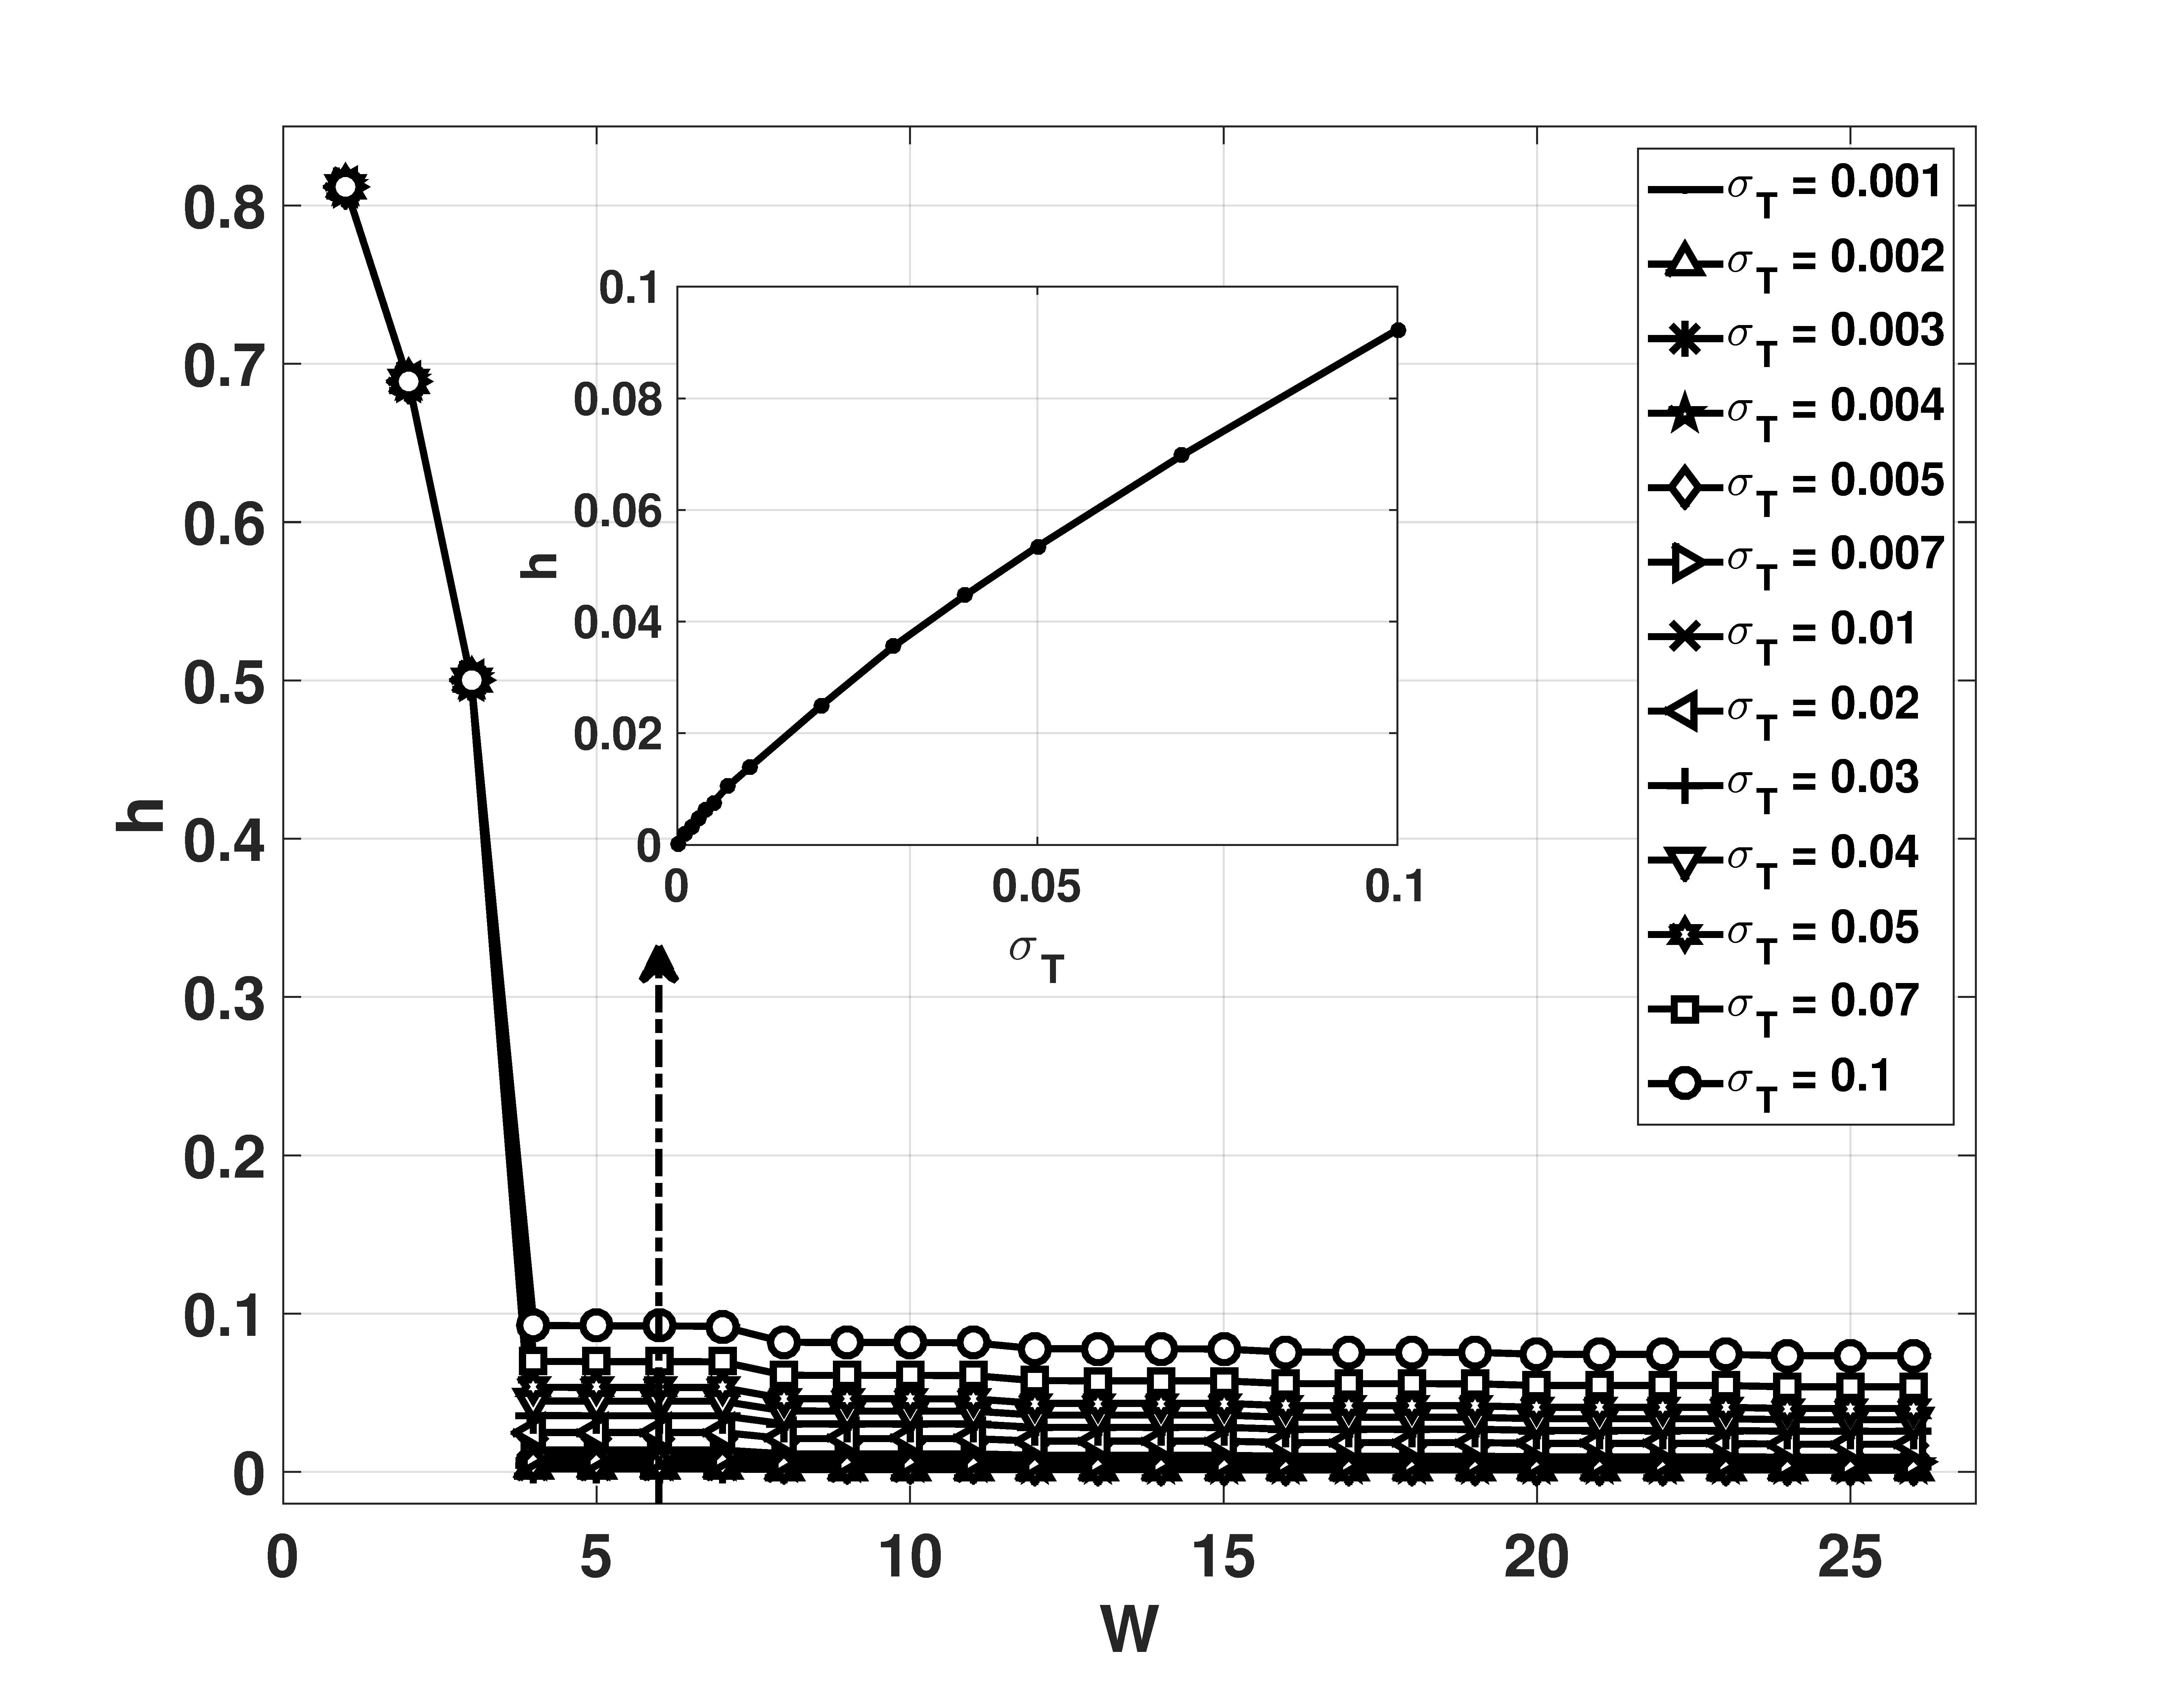
\includegraphics[ width=0.8\textwidth]{h_W_CJ}
\caption{$h$ as a function of $W$ for a \emph{RO} sampled with $r=8$, for jitter with several variances. The inset shows $h$ as a function of $\sigma_T$ for $r=8$ and $W=6$.}
\label{fig:h_W_CJ}
\end{figure}

\begin{figure}
\center
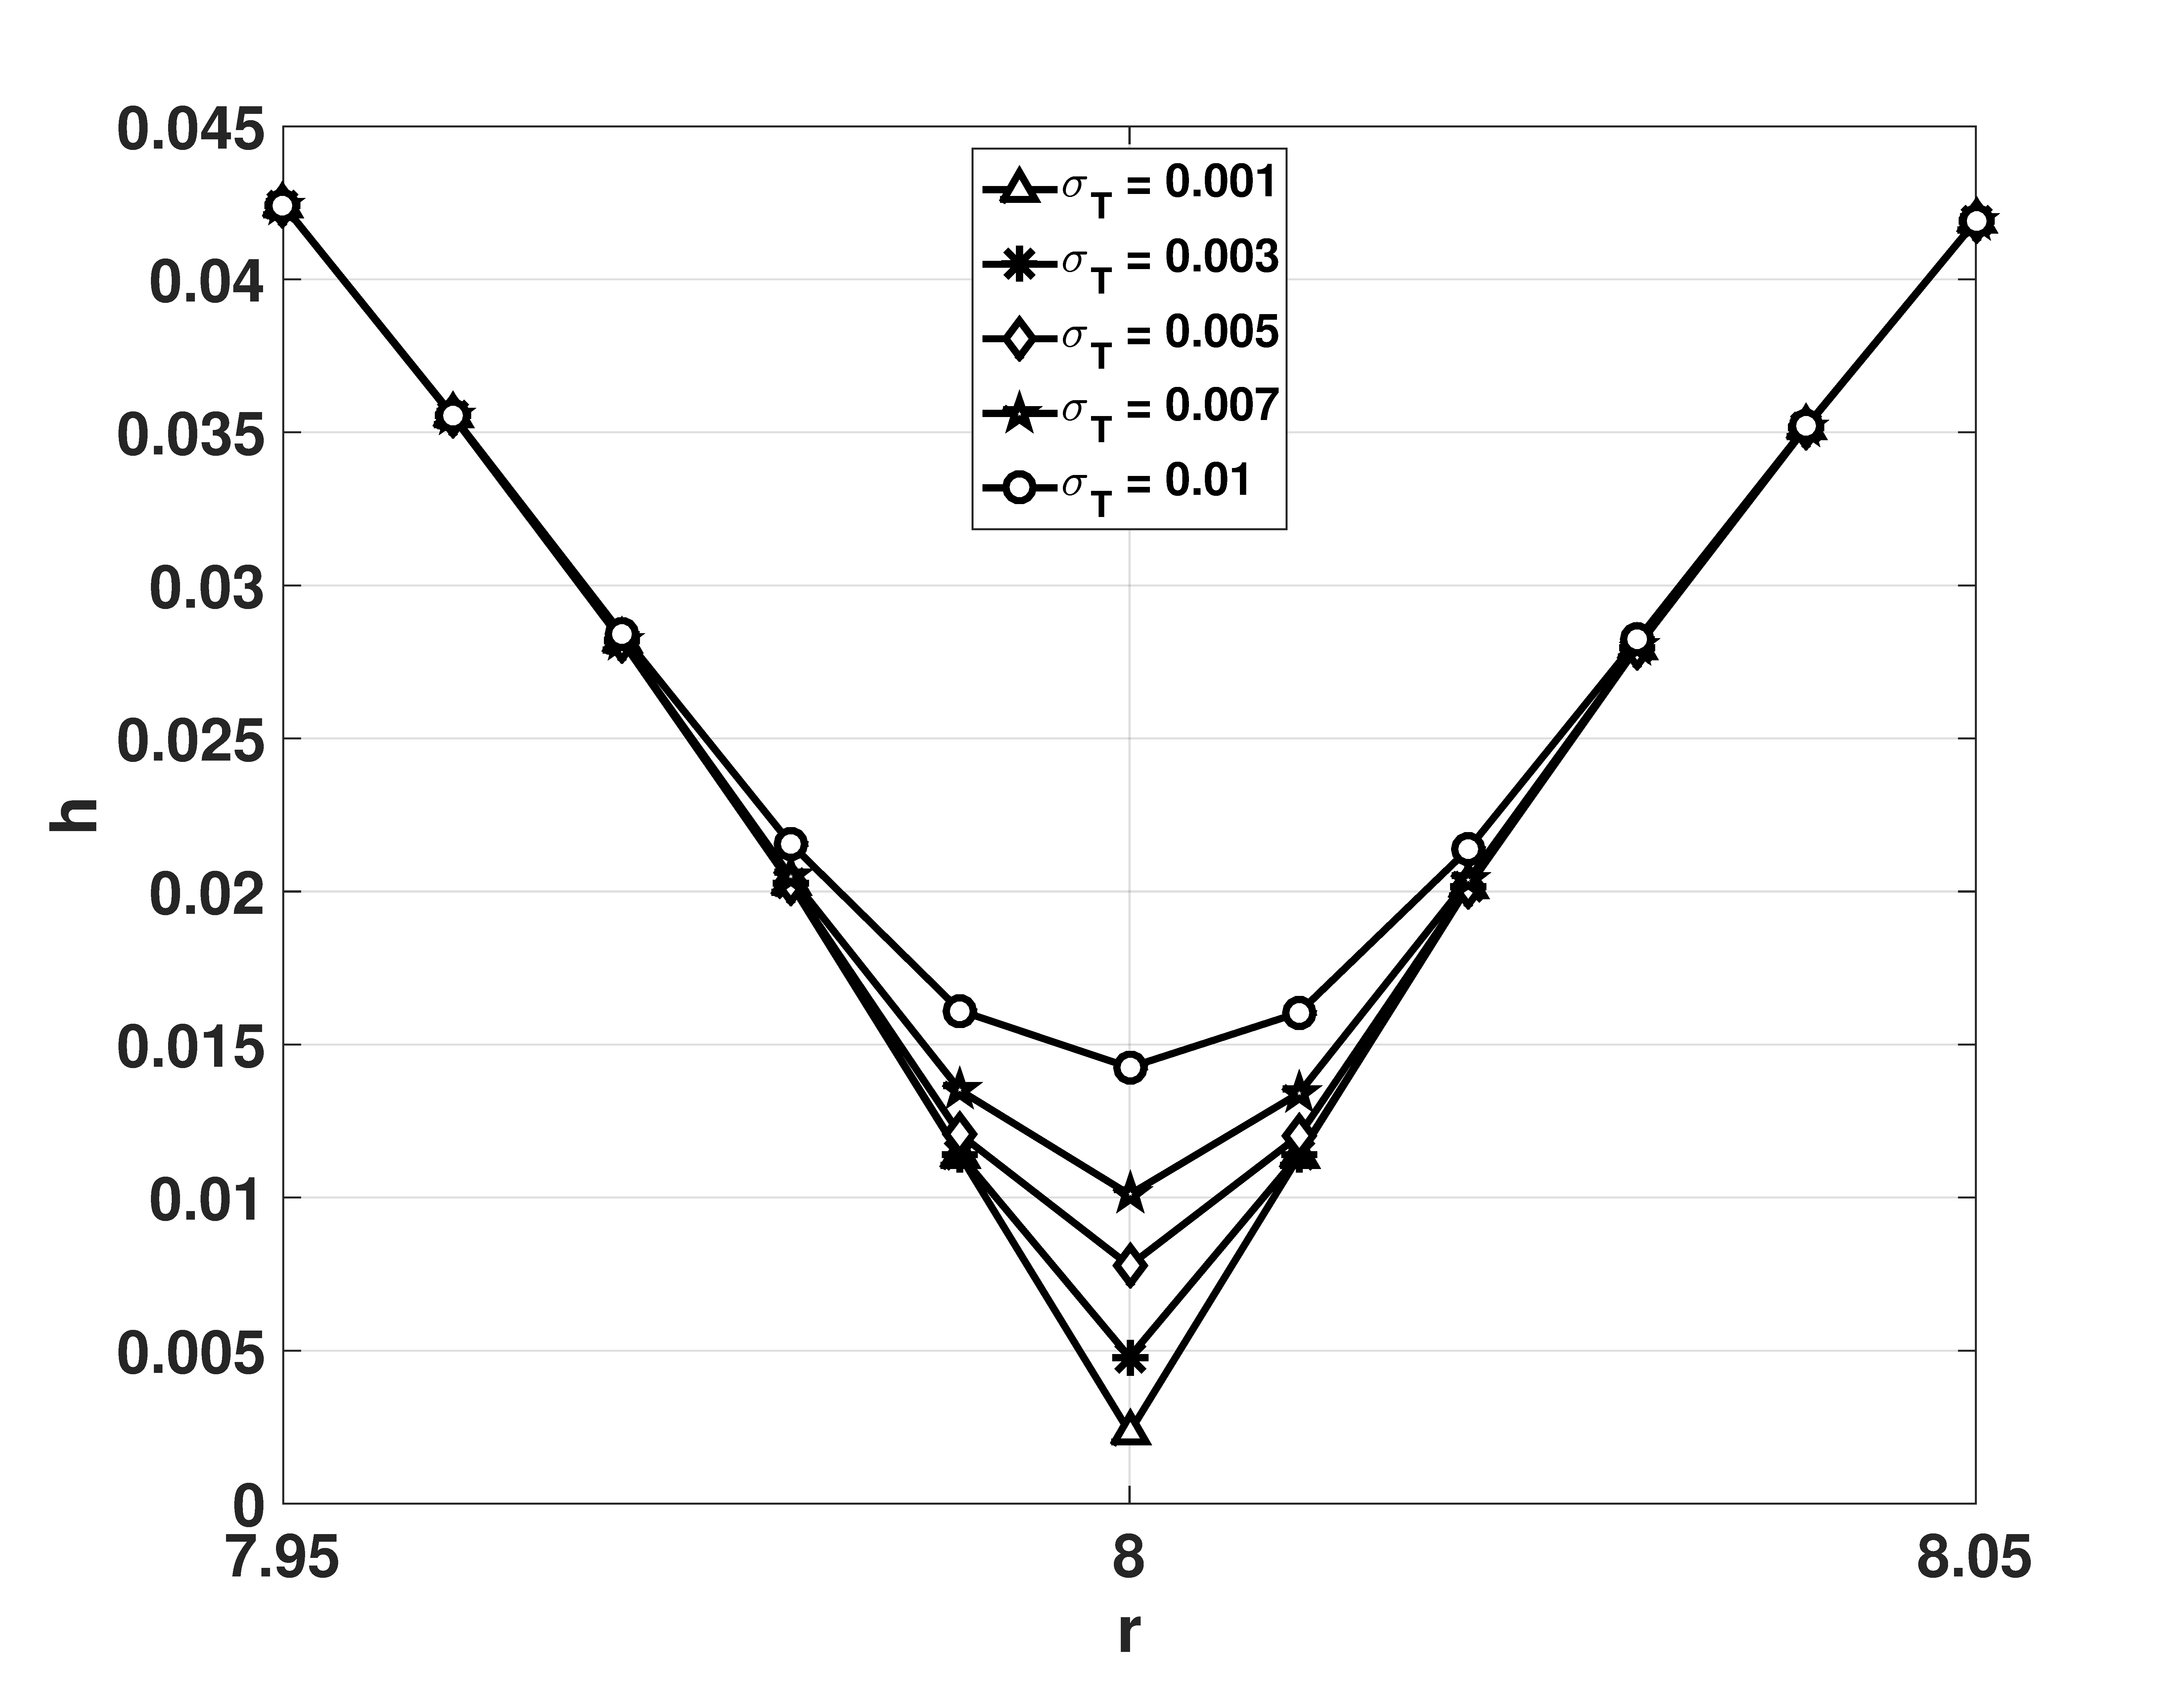
\includegraphics[ width=0.8\textwidth]{h_r_CJ}
\caption{$h$ as a function of $r$ for $r\in[7.95,8.05]$, with several $\sigma_T$ and $W=6$ . The curve has a minimum at the optimum value $r=8$.}
\label{fig:h_r_CJ}
\end{figure}

Further analysis must be done to assure that the selected values $W=6$ and $D=8$ produce symbolic files with a good statistics. For a given alphabet $\mathcal{A}$ with $m$ elements, and a given symbolic file of length $n$, the quality parameter $\alpha=n/m$, see \ref{sec:quanti}. Quality is better as $\alpha$ increases and a minimum value $\alpha=10$ was accepted. According to section \ref{sec:quanti} the selected values $W=6$ and $D=8$ provide $\alpha_h\simeq10^5$, $\alpha_{h^*}\simeq175$ with superposition and $29$ without superposition. All cases give $\alpha>10$ as required.

%PARTE DE ESTO TIENE QUE IR A LA SECCION CUANTI


%============= el que sigue es el plano general y me parece que es mejor no ponerlo =============================================================
%Figure \ref{fig:hm_h_CJ} shows the $h^*_{m}-h}$ plane. The quantifiers have been calculated sweeping the values of $D$ from $2$ to $11$, and $W$ from $2$ to $26$ (both for $h^*$ and only $W$ in the case of $h_{hist}$).
%Better differentiation is obtained for higher values of the parameters, this is because both quantifiers tend to quantify the source value for $D$ and $W$ equal to infinite.
%Nevertheless, this is impossible in real practice, also the amount of data available limits the values of the parameters based to achieve good statistics. Therefore, we seek the minimum values (threshold value) of the parameters that discern the jitter good enough. In Figure \ref{fig:hvsh_8} it can be seen that for values of $W$ equal to $3$ or lower the $h_{hist}$ quantifier is insensitive to the variations of the jitter. Therefore, $W$ should be $4$ or higher, this result is in concordance with the threshold determined in Figures \ref{fig:hhistvsW_T8_CJ}. In the case of $h^*$ the $W$ value should be equal or higher than $4$ and the value of $D$ higher than $7$, again this result is in concordance with the ones derived from Figures \ref{fig:hmvsD_T8} and \ref{fig:hmvsD_CJ_T8}. The bottom left area of the plane is the one with better performance of both quantifiers.
%========== fin plano general

A comparison between both quantifiers is shown in Figure \ref{fig:hm_h_CJ}. Markers correspond to variances $\sigma_T=\{0,$ $0.001,$ $0.002,$ $0.003,$ $0.004,$ $0.005,$ $0.007,$ $0.01,$ $0.02,$ $0.03,$ $0.04,$ $0.05,$ $0.07,$ $0.1\}$.
Note that the slope of any of these curves is $dh^*/dh$ and it is equal to the quotient between slopes of curves in the insets of Figs. \ref{fig:hm_D_CJ}, and \ref{fig:h_W_CJ}. If $dh^*/dh~>1$, $h^*$ is more sensitive than $h$ to measure jitter. The slope slightly increases from $\sim2.47$ for $W=5$ to $\sim5.54$ for $W=19$ showing that $h^*$ becomes more sensitive as $W$ increases.

\begin{figure}
\center
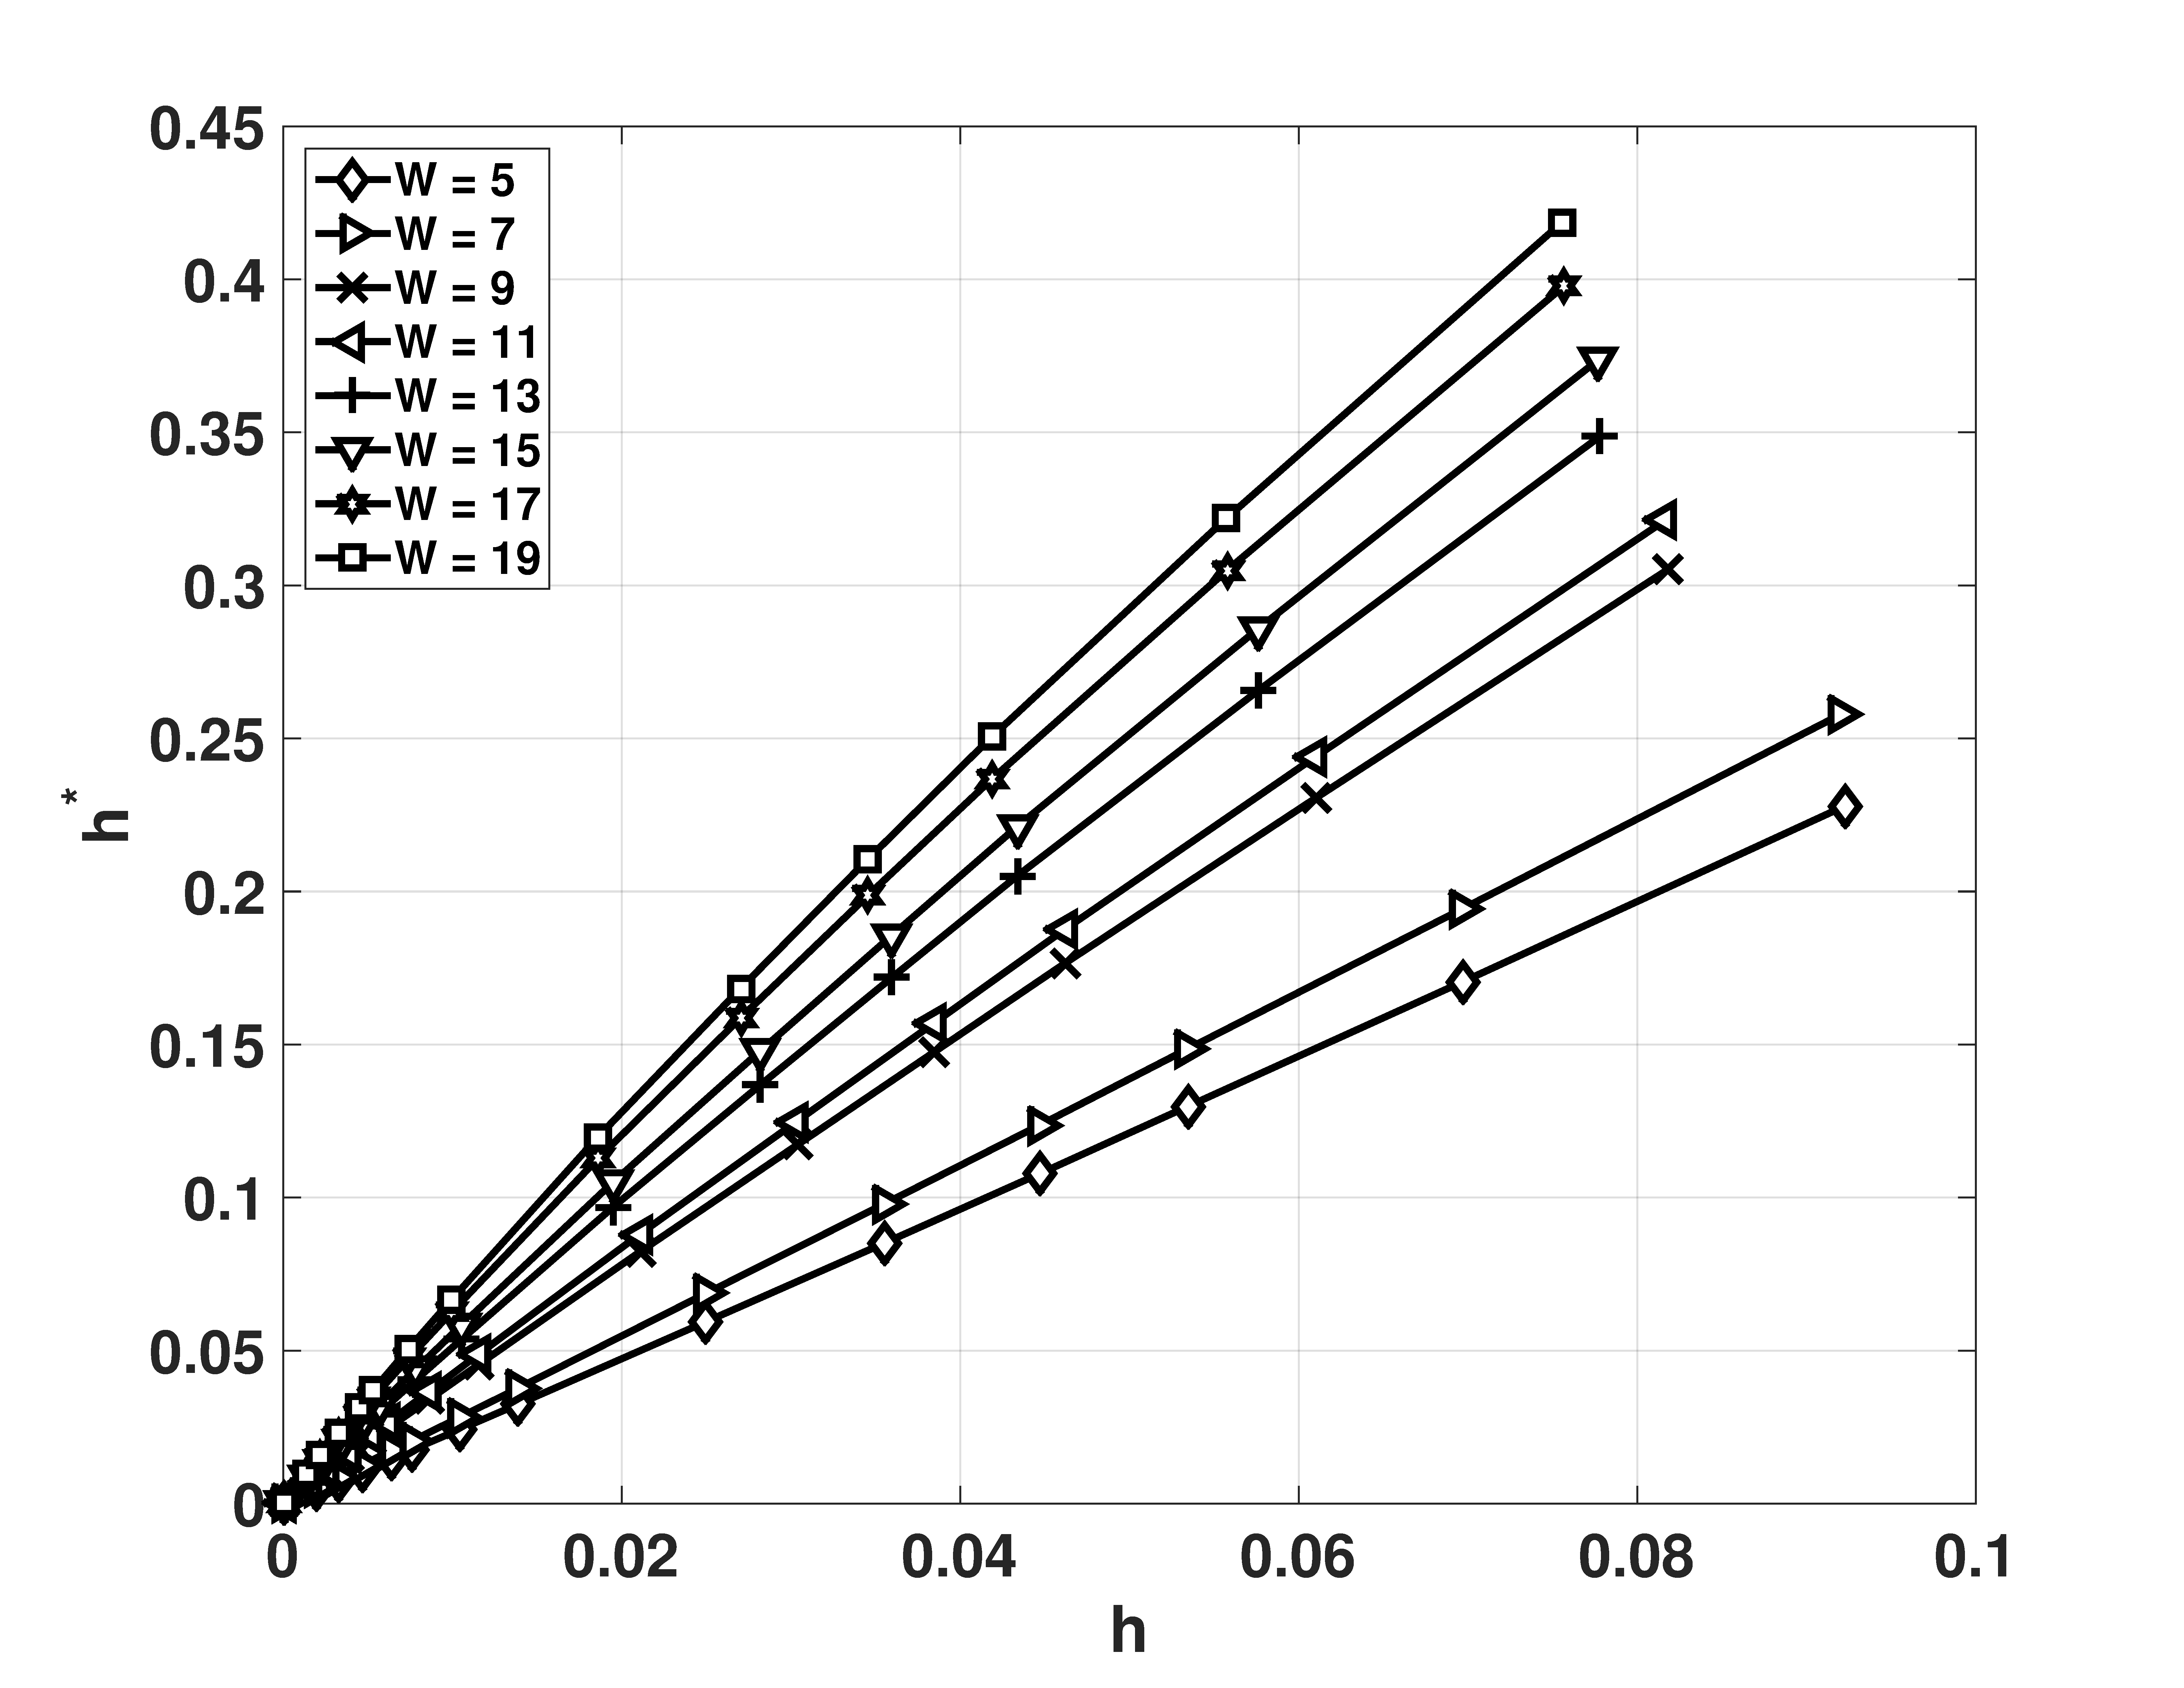
\includegraphics[ width=0.8\textwidth]{hm_h_CJ}
\caption{$h^*$ as a function of $h$ for $r=8$, $D=8$ and different values of $W$.}
\label{fig:hm_h_CJ}
\end{figure}

%Further sensitivity improvement may be obtained by making a minor change in the evaluation of $h^*$: the procedure starts converting blocks of $W$ consecutive bits into natural numbers between $0$ and $2^W$. Each block may have or not a superposition with the previous one. Then $D$ consecutive natural numbers are used to obtain an ordering pattern. Again these step may be done with or without superposition. In the calculations reported in previous Figs. there are $W-1$ bits shared between consecutive blocks and $D-1$ numbers shared between consecutive ordering patterns.

We also evaluated $h^*$ without the superposition of bits between consecutive natural numbers but keeping the superposition of $D-1$ natural numbers between ordering patterns (In all cases $h$ was evaluated with superposition of $W-1$ consecutive bits). Results are depicted in Fig. \ref{fig:Deltahm_Deltah_CS_SS} where it is shown that removing the superposition the sensitivity of this quantifier increases. Of course, we get a smaller amount of $W$ bits natural numbers form the original seven million binary file, and consequently, the statistical quality is lower than that of the original calculation with superposition. To increase $\alpha$ up to its previous value, longer binary files are required.

\begin{figure}
\center
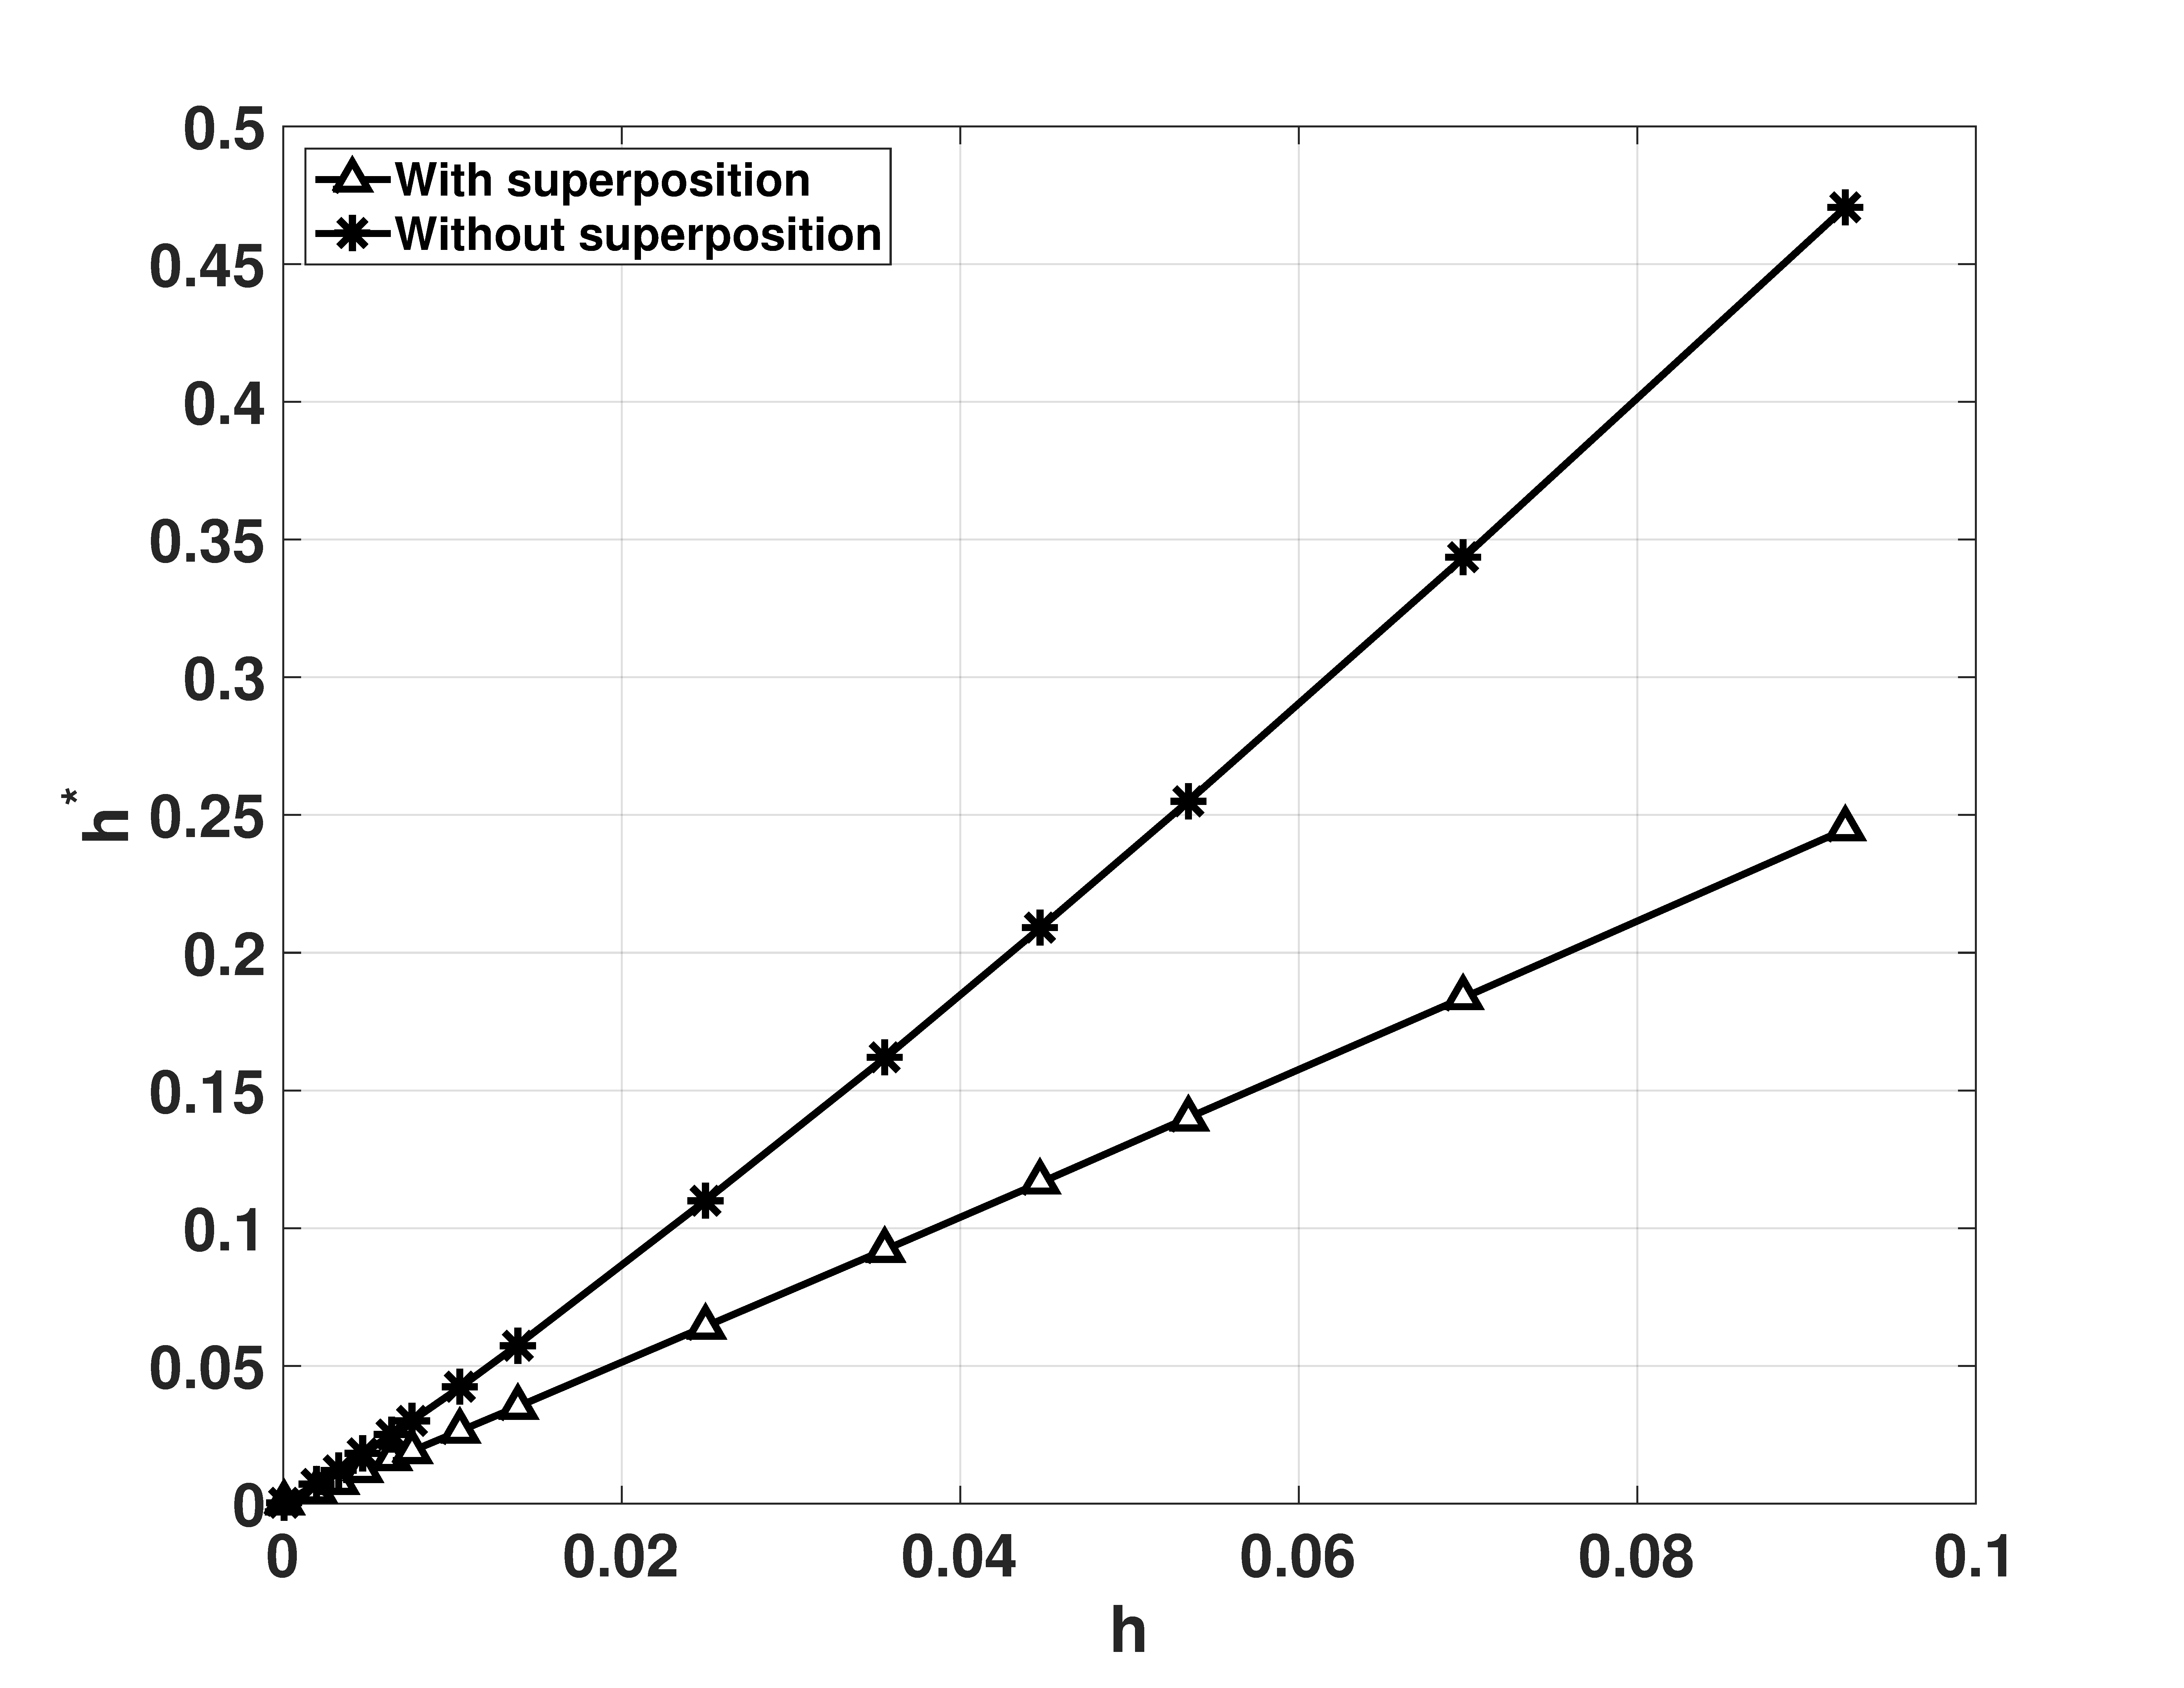
\includegraphics[ width=0.8\textwidth]{Deltahm_Deltah_CS_SS}
\caption{$h^*$ as a function of $h$ for $r=8$, $W=6$ and $D=8$. Two procedures to obtain $W$-bits natural numbers are considered: with and without superposition (see text).}
\label{fig:Deltahm_Deltah_CS_SS}
\end{figure}